\chapter{Comparing D$_2$-glucose and D$_7$-glucose in DMI}
\label{Chap:Glucose}

\section{Introduction}

\ac{DMI} is a \ac{MRSI} method that enables substrates and metabolic products that are labelled with the non-radioactive hydrogen isotope $^2$H, to be mapped \textit{in vivo}. The scientific impact of $^2$H and usage in the real world has increased greatly since its existence was first theorised \cite{Urey1932AConcentration}, and it was not long before its potential for biological applications was recognised \cite{Schoenheimer1935DeuteriumMetabolism, Schoenheimer1938TheMetabolism}. Of particular interest is the use of glucose as the administered labelled precursor molecule, as this provide a direct probe of glucose metabolism. Whilst the most common current uses for $^2$H for \textit{in vivo} \ac{NMR} measurements involve deuterated glucose, initially it was \ac{D$_2$O} that was ingested to elevate $^2$H levels for use in \ac{NMR} \cite{Brereton1986PreliminarySpectroscopy, Irving1987InSpectroscopy}, to investigate lipid metabolism. The most useful forms of deuterated glucose are those whose carbon-bonded hydrogen atoms in the first and sixth positions have been replaced by deuterium because these substitutions are the only ones that are transferred to pyruvate, and then to either lactate (Lac) or to a combination of glutamate and glutamine (Glx) via the \ac{TCA} cycle in the mitochondria. For this reason, [6,6'-$^2$H$_2$] glucose has been a common choice of labelling (isotopologue), providing twice the number of $^2$H labels as would [1-$^2$H] glucose, and it has been used in many \textit{in vivo} studies ranging from preclinical work \cite{Lu2017QuantitativeSpectroscopy, Meerwaldt2023InImaging} to demonstration in humans  \cite{DeFeyter2018DeuteriumVivo, Roig2022Deuterium7T}. Lactate and Glx as well as non-metabolised glucose and water (\ac{NA} plus an additional amount caused by label-loss during various processes) become detectable via either choice of labelling. The detected lactate and Glx provide information about the tissue’s propensity to metabolise glucose via glycolysis or the oxidative phosphorylation pathway, and thereby an important clinical potential of DMI is identified since many tumour cells exhibit an increased tendency for glycolysis. This manifests in higher than usual lactate production;  the well-known Warburg effect \cite{Warburg1956OnCells}.    

$^2$H \ac{NMR} measurements following labelled glucose ingestion or injection allows information on downstream metabolite concentrations to be quantified as well as tracked to obtain metabolic flux measurements, without the use of ionising radiation. In contrast \ac{PET} scans using \ac{FDG}  involve ionising radiation and only provide information on glucose uptake. Besides th effect of cancer and other disease states, brain metabolism is also altered locally, albeit temporarily, as part of normal function. This might occur when a part of the brain is activated by a task or stimulus, such as by visual stimulation. For example it has been previously shown many times that there is metabolic activation in the visual cortex following visual stimulation \cite{Kushner1988CerebralStimulation, Beland-Millar2018FluctuationsStimulation}. Using $^1$H \ac{MRS} lactate increases \cite{Prichard1991LactateStimulation., Sappey-Marinier1992EffectSpectroscopy, Fernandes2020MeasurementT}, and glucose decreases \cite{Lin2012InvestigatingT} in the visual cortex following visual stimulation have been measured. $^{13}$C \cite{Chhina2001MeasurementSpectroscopy} \ac{MRS} has been used to measure TCA activation in the voxel cortex, and $^{31}$P \ac{MRS} has been used to measure signal changes in lactate, phosphocreatine and inorganic phosphate in the visual cortex \cite{Sappey-Marinier1992EffectSpectroscopy} glucose signals are not present in these measurments. It is important to note that significant increases in glutamate (2\%) and decreases in glutamine (8\%) have also been shown \cite{Lin2012InvestigatingT}.
 
In its simplest form, \ac{DMI} is relatively straightforward to implement using a pulse-acquire \ac{CSI} sequence, usually without the need for water suppression because of the low concentration of naturally occurring deuterated water. In most cases, the \ac{DMI} spectra are also simpler to analyse than the proton spectra. If using glucose as the labelled substrate, there are just four metabolites to consider: water (\ac{HDO}), glucose, Glx, and lactate. This relative simplicity can be regarded as a positive attribute in the context of potential clinical translation. However, the generally low \ac{SNR} of \ac{DMI} is not a favourable characteristic, and means that data is often acquired with low spatial resolution, often with voxels of around 8 ml \cite{DeFeyter2021DeuteriumFuture, deGraaf2020OnImaging} in volume; the smallest reported voxel size to date in humans is 2.97 ml \cite{Ruhm2022Dynamic9.4T}, in measurements made at a high magnetic field strength of 9.4 T. Low \ac{SNR} and spatial resolution can potentially be improved upon by performing \ac{DMI} scans through indirect detection using $^1$H \ac{MRSI} \cite{vanZijl2020SpectroscopicFluxes, Bednarik2021DeuteriumBrain, Niess2023Reproducibility3T, Ruhm2022Dynamic9.4T}. This has the benefit of not requiring deuterium-specific hardware, but this comes at the expense of often requiring a more complex acquisition scheme and post-processing analysis. Another method of increasing \ac{SNR} in \ac{DMI} is to implement de-noising during post-processing analysis, this has been shown to improve \ac{SNR} in \ac{MRSI} using low rank approximations \cite{Nguyen2013DenoisingApproximations}. Similar techniques using Tucker decomposition \cite{Tucker1966SomeAnalysis, Bader2007EfficientTensors} have been applied to \ac{DMI} data with notable \ac{SNR} improvements \cite{vonMorze2021ComparisonT, Kreis2020MeasuringMRI}.

\begin{figure}
    \centering
    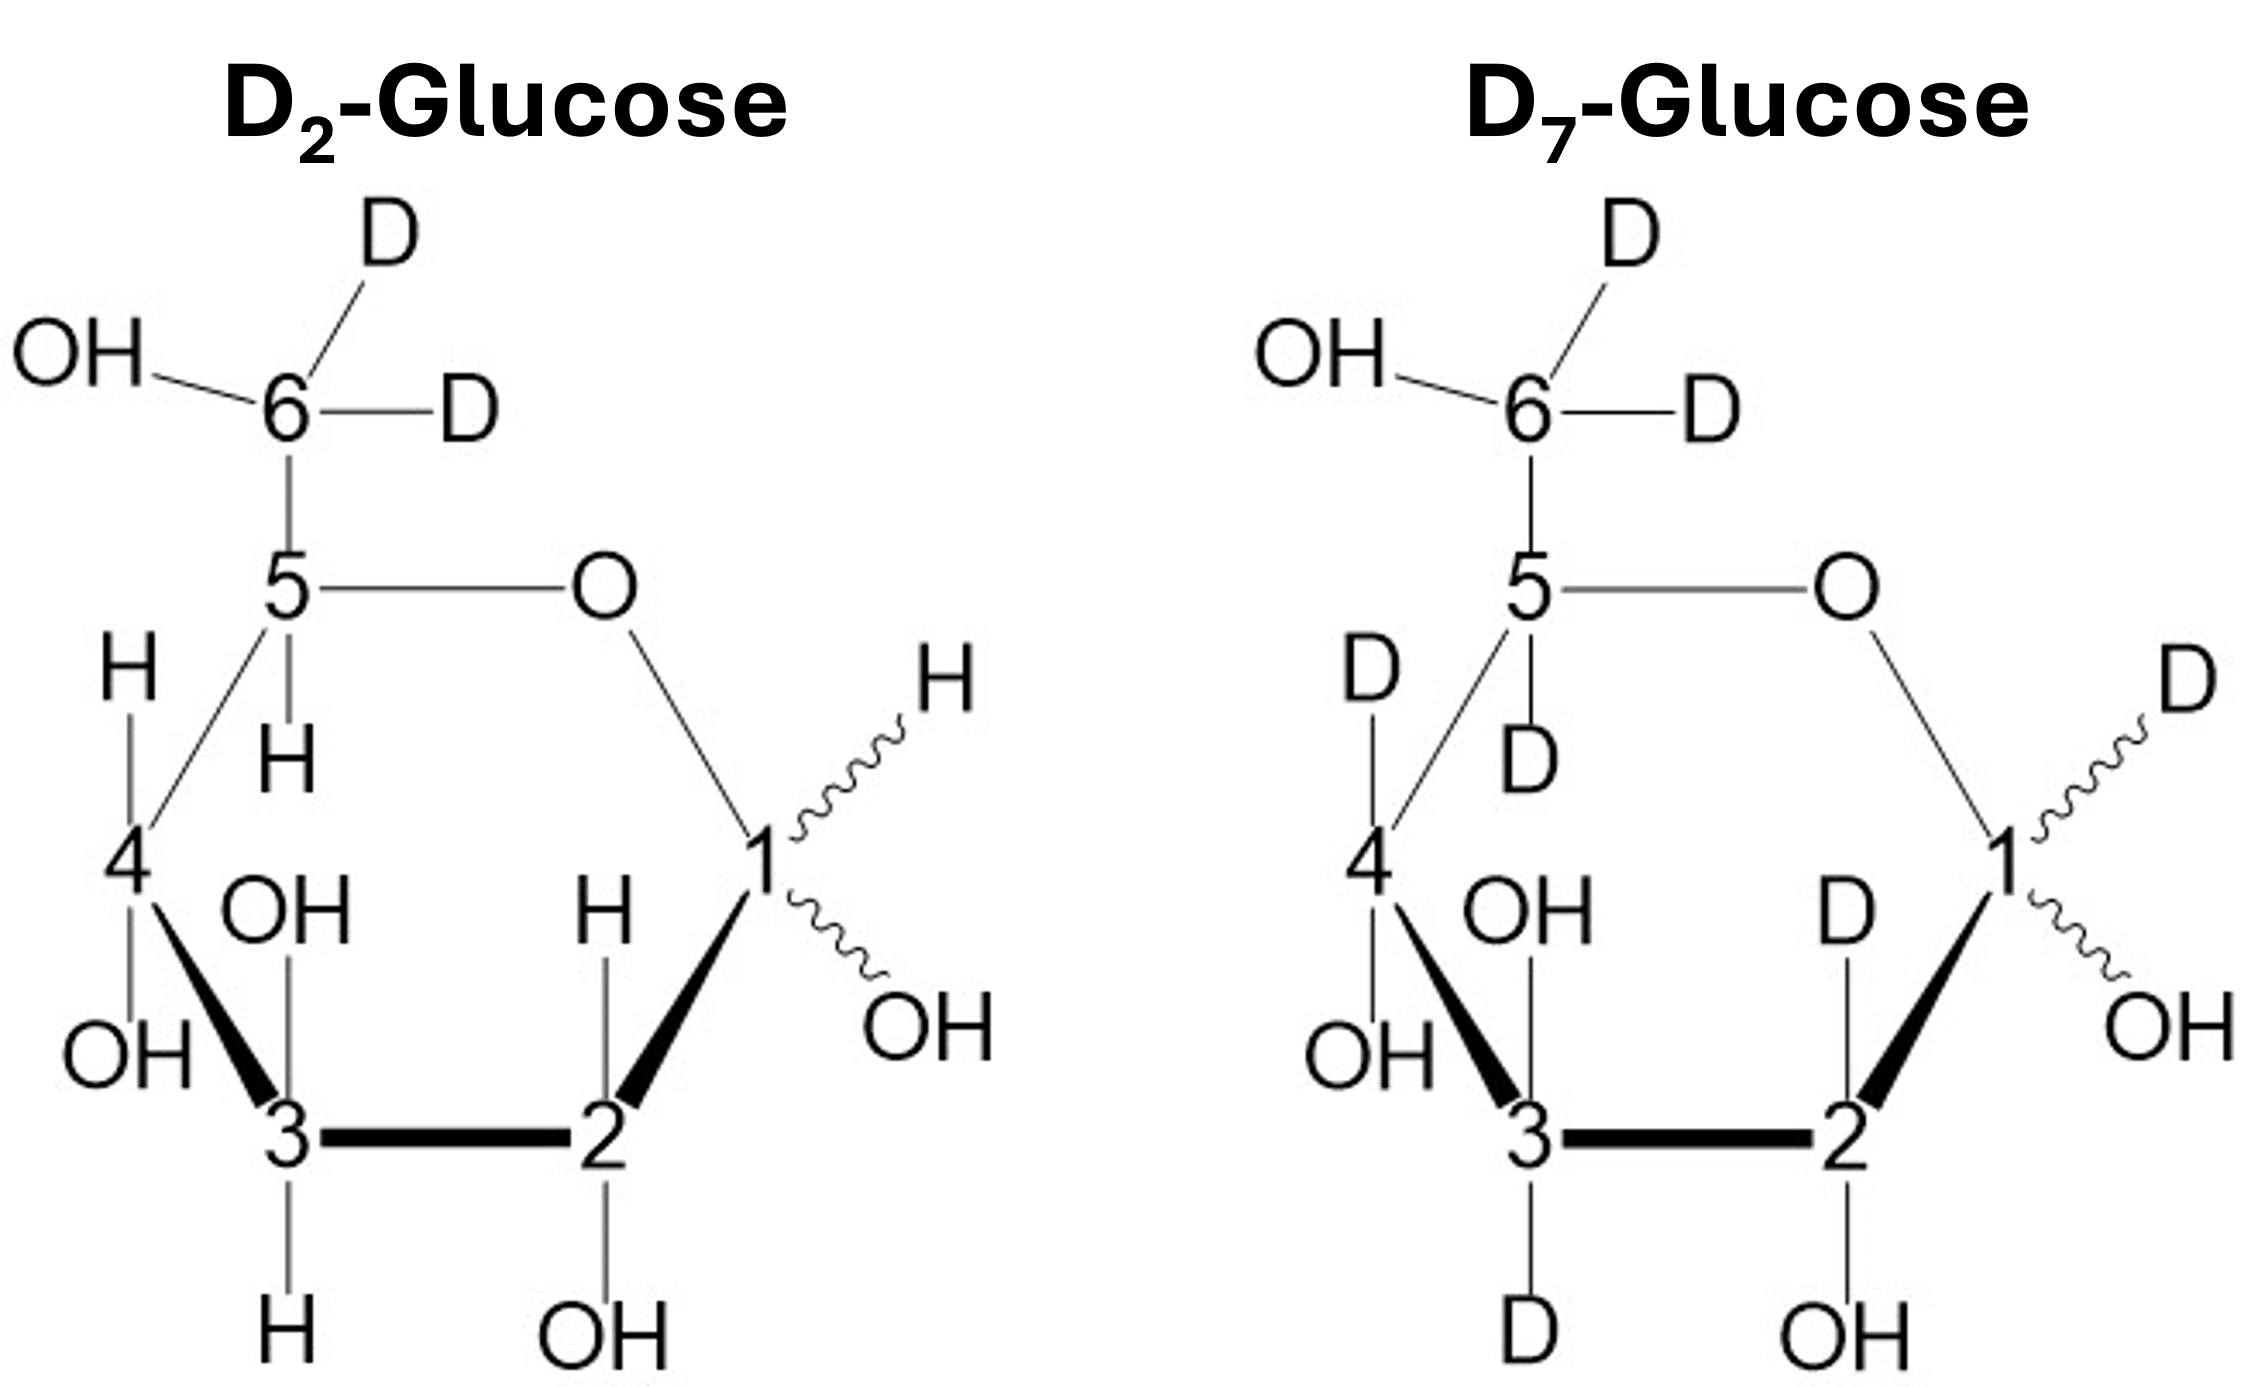
\includegraphics[width = 1\textwidth]{Figures/Glucose/Glucose.png}
    \caption{\textit{The chemical structure of D$_2$ (left) and D$_7$-glucose, where D represents deuterium atoms and each number represents a carbon atom with the number referring to the position.}}
    \label{fig:Glu:Glucose}
\end{figure}

Other labelled compounds then D$_2$-glucose have also been used to investigate \textit{in vivo} metabolism in conjunction with \ac{DMI}. For example [6,6'-$^2$H$_2$] fructose has been used to investigate liver cancer \cite{Zhang202366-2H2Cancer}. Fructose was found to have a similar spectral appearance as the glucose, with slightly different kinetics. Intravenous injection of deuterated acetate ([$^2$H$_3$] acetate) has been used to investigate myocardial metabolism \cite{Wang2021NoninvasiveImaging} and tumour metabolism \cite{DeFeyter2018DeuteriumVivo}, where acetate accumulation and Glx changes were tracked.

One important way of increasing the $^2$H signal is to use a form of deuterated glucose with a larger number of $^2$H labels. Since there are twelve hydrogen atoms in the glucose molecule, all twelve could be substituted with $^2$H atoms. However, those atoms in the hydroxyl groups rapidly exchange rapidly with the surrounding water and therefore are not usually useful in metabolic applications. The seven other locations in which the $^2$H atoms are directly carbon-bonded are less labile and potentially useful labelling sites, yielding the form [1,2,3,4,5,6,6'-$^2$H$_7$]-glucose (D$_7$-glucose). Compared with [6,6'-$^2$H$_2$]-glucose (D$_2$-glucose), the $^2$H spectrum of D$_7$-glucose would contain a factor of 7/2 times more components, many of which overlap due to the broad linewidths of $^2$H, thus producing a gain in \ac{SNR}. The $^2$H atoms in the C1 and C6 positions (in the absence of label-loss) will be transferred to lactate or Glx molecules \cite{DeFeyter2020DeuteriumBrain}, producing a gain of 3/2 in the Glx signal. A similar gain is expected for lactate. Therefore, it is expected that the use of D$_7$-glucose will increase the \ac{SNR} and reliability of detected signals for glucose, Glx, and lactate, compared to using D$_2$-glucose. In addition, the four remaining $^2$H labels in the positions C2, C3, C4 and C5 of D$_7$-glucose are transferred directly or indirectly to water during glycolysis, and will therefore contribute to an increased \ac{HDO} signal \cite{Mahar2020HDOMetabolism, Mahar2021DeuteratedGlucose}. The \ac{HDO} (deuterated water) signal increase that is a result from metabolism has been shown to be directly proportional to the increase in downstream metabolites (Glx and lactate) \cite{Mahar2021DeuteratedGlucose}, which implies that regular non-spectroscopic imaging of the \ac{HDO} signal increase could be used as a measure of the Warburg effect potentially providing improved spatiotemporal resolution compared to \ac{MRSI} techniques. 

The primary aim of this study is to measure the difference in vivo metabolite signal/concentration changes for \ac{HDO}, glucose, Glx and lactate in the brains of healthy human participants following ingestion of D$_2$-glucose or D$_7$-glucose. This the first instance of D$_7$-glucose being used with human subjects. Each participant drank 250 ml of water containing 0.75g/kg of of dissolved labelled glucose. \ac{CSI} scanning, de-noising and a sophisticated and robust fitting routine was used to track the change in metabolite signals. Metabolite signals for each metabolite were found to be larger for all metabolites after ingestion of D$_7$-glucose, concentration values were also found to be larger in each metabolite except glucose. Secondarily, the possibility of detecting differences in metabolite concentrations due to an applied visual stimulus was investigated.  

\section{Methodology}

\subsection{Particicpants}

Scanning was performed on a 7T Achieva scanner (Philips Healthcare), operating at 45.8 MHz for $^2$H. A 26.4 cm inner-diameter, dual-tuned $^1$H/$^2$H birdcage \ac{RF} coil (Rapid Biomedical) was used for $^2$H measurements and anatomical $^1$H images. Ethical approval was received from the Faculty of Medicine and Health Sciences Research Ethics Committee (ref. no. FMHS 306-0621) at the University of Nottingham to recruit 15 healthy participants for this study. Informed consent was received from all participants who were only recruited if they had: a \ac{BMI} $<$ 25 kg/m$^2$ (or less than 27 kg/m$^2$ for males whose waist circumference was $<$94 cm), had a normal heart rate and blood pressure, a blood glucose concentration of $<$7.8 mM (finger-prick test), an age between 18 and 60 years, and no significant medical conditions or issues related to safety in the MR scanner. As participants are being given extra glucose it is important to minimise the risk hyperglycaemia, which is why participants that are at risk of developing type-2 diabetes are excluded. Older participants and those taking oral medication are excluded as their metabolism can be altered. At the screening visit, participants were informed whether visual stimulation would be applied and that at least an eight hour fast would be required on the day of scanning. Blood glucose status was checked using a second blood glucose level test (finger-prick) that had to be $<$5.6 mM. For those receiving D$_2$-glucose (n=8), 5 experienced a visual stimulus. For those receiving D$_7$-glucose (n=7), 4 experienced a visual stimulus.

\subsection{Scan Protocol}

\begin{figure}
    \centering
    
\includegraphics[width = 1\textwidth]{Figures/Glucose/Scan_Details.png}
    \caption{\textit{The parameter details for each of the scans used in this study. Note that the averages for CSI are acquisition weighted, and that the 'Bulk' spectra is non-localised.}}
    \label{fig:Glu:Scan_Details}
\end{figure}

Scanning for each participant was split into two parts, the baseline \ac{NA} scanning before the glucose drink (lasting approximately 20 minutes) which are used for quantification and calibration, and the 90-minute scanning session after the glucose drink was ingested. The drink was consumed in a maximum of eight minutes. Baseline measurements included a $^1$H scout scan for planning; a $^1$H \ac{MPRAGE} scan (\ac{FOV}: 224 x 224 x 140 mm$^3$, 1.4 mm isotropic voxels, \ac{TR}: 7.1 ms, \ac{TE}: 2.6 ms, T$_\text{scan}$: 353 s); a non-localised $^2$H spectrum (16 averages, \ac{TR}: 1000 ms, \ac{TE}: 1.1 ms, $\alpha$: 90$^\circ$, \ac{BW}: 3000 Hz, 2048 samples, with a scan duration of 17 s); a slice-selective $^2$H spectra, acquired from a 2-cm-thick axial slice positioned over the lateral ventricles, using 128 averages, TR: 1000 ms, TE: 1.9 ms, $\alpha$: 90$^\circ$, \ac{BW}: 3000 Hz,  2048 samples with a T$_\text{scan}$: 129 s and a 3D $^2$H \ac{CSI} covering the whole brain (\ac{FOV}: 180 x 180 x 120 mm$^3$ , 15 mm isotropic voxels, \ac{TR}: 230 ms, \ac{TE}: 2.4 ms, $\alpha$: 62$^\circ$, \ac{BW}: 1200 Hz, 256 samples, with a T$_\text{scan}$: 670 s) acquired using 6 acquisition-weighted \cite{Pohmann2001AccurateCSI} averages. All the \ac{NA} scans were performed in the absence of visual stimulation and after these data were acquired the participant was then brought out of the scanner and consumed the glucose drink. This contained 0.75g/kg (bodyweight) of either D$_2$ or D$_7$-glucose powder purchased from CK Isotopes Ltd. (microbiological/pyrogen-tested product) and Merck Life Science UK Ltd. (endotoxin-tested product) dissolved in 250 ml of water at room temperature. The participant was allowed to consume this in their own time, and when they indicated that they were ready for the second scanning session ($\sim$30 minutes later), were guided back into the scanner.

\begin{figure}
    \centering
    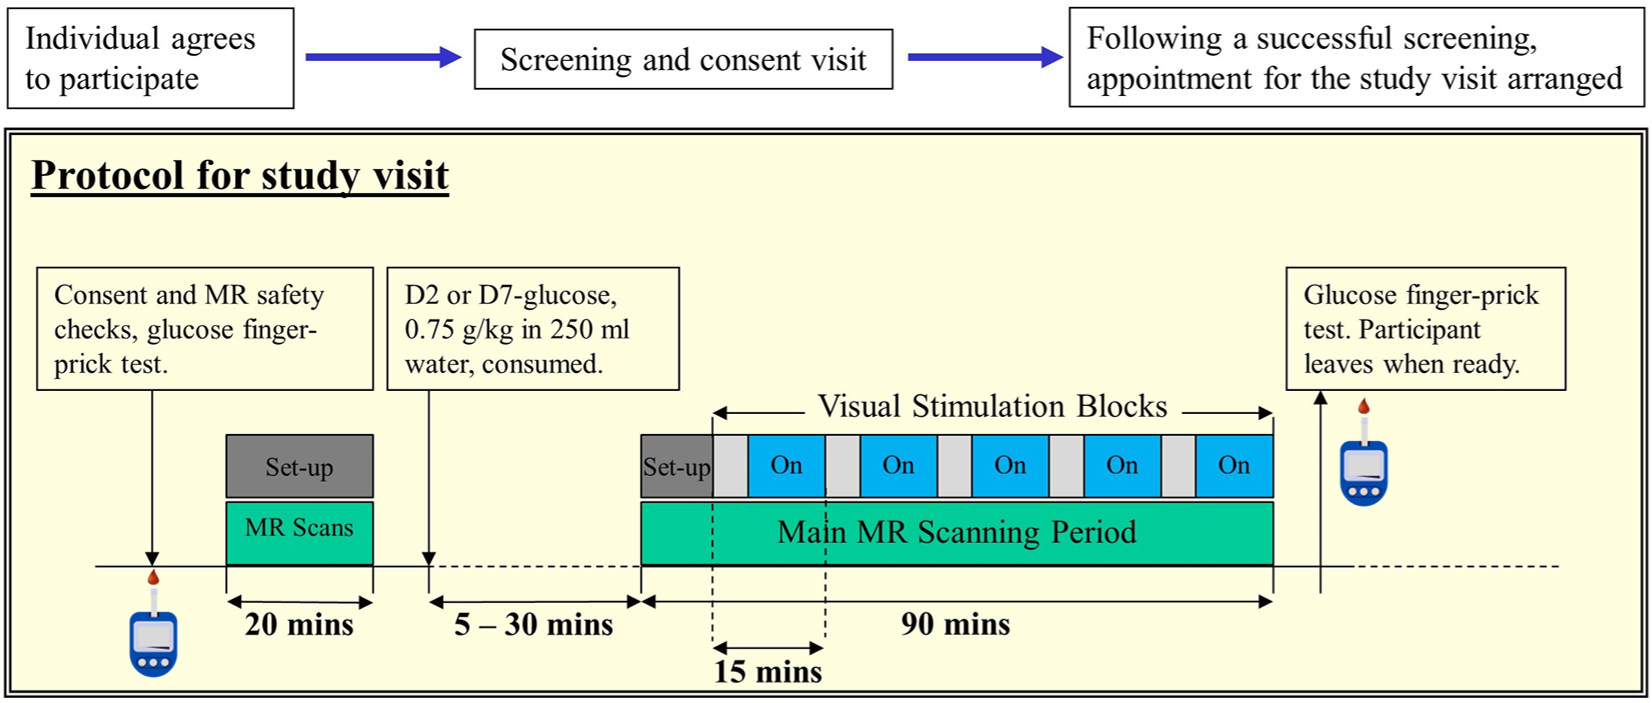
\includegraphics[width = 1\textwidth]{Figures/Glucose/Protocol.png}
    \caption{\textit{Schematic of the scanning protocol that was used in this study.}}
    \label{fig:Glu:Protocol}
\end{figure}

In the second session, the two $^1$H scans were repeated, followed by five or six repeats of the three $^2$H scans. In the event that the participant needed to exit the scanner for a short period and re-enter, the $^1$H scans were repeated before continuing with the $^2$H scans. If the participant was to be visually stimulated, the display was activated during the \ac{CSI} scans only and quiescent otherwise.  

Visual stimulation was produced via an 8 Hz flashing, black and white, radial checkerboard, similar to what has been used previously \cite{Fernandes2020MeasurementT}. The visual display was projected onto a screen that the participants could observed by wearign prism glasses while lying in the scanner. Most of the participants who experienced visual stimulation (three that ingested D$_2$-glucose and four that ingested D$_7$-glucose) were shown a checkerboard flashing pattern that was active for 50 seconds followed by 10 seconds of presentation of a red cross on a grey background. However, two participants (both of whom ingested D$_2$-glucose) experienced a checkerboard flashing pattern that was active for 30 seconds followed by 30 seconds of a red cross on a grey background. Participants who received no visual stimulation were asked to close their eyes durig the scanning session. In all cases, the scanner room lights were turned off. 

\subsection{Image and spectral processing}

\begin{table}[H]
    \centering
    
\includegraphics[width = 1\textwidth]{Figures/Glucose/Prior_Table.png}
    \caption{\textit{Table that includes the prior knowledge used to fit the individual \ac{CSI} datasets after D$_7$-glucose ingestion, which includes the parameters chemical shift, linewidth, amplitude and phase. The acronyms are defined as LB:Lower-Bound, UB:Upper-Bound and IV:Initial-Value. N/a refers to non-applicable meaning the parameter is not sued with this metabolite, this is because it is grouped to something else or is not grouped to any other metabolite Computationally n/a is used as an empty matrix ([]). The 'G' column shows which peaks are grouped for each parameter.}}
    \label{fig:Glu:Prior}
\end{table}

The $^1$H \ac{MPRAGE} images were converted to a NIFTI format using MRIcroGL (www.nitrc.org), and bias-field corrected using FSL-FAST \cite{Zhang2001SegmentationAlgorithm}. The corrected \ac{MPRAGE} image was then brain extracted using FSL-BET \cite{Smith2002FastExtraction} which also bias-field-corrected the image and removed any neck voxels. The fractional intensity threshold was allowed to vary between subjects along with the gradient in the foot head direction, this was to make sure the brain extraction was optimised for each participant. The MNI-152 brain image with 2 mm isotropic voxels (distributed with FSL \cite{Smith2004AdvancesFSL}) was linearly registered to each image using FSL-FLIRT \cite{Jenkinson2001AImages, Jenkinson2002ImprovedImages} and twelve degrees of freedom. The MNI-152 brain image was then non-linearly registered to the same image to obtain the warp-field using FSL-FNIRT \cite{AnderssonJ2008FNIRT-FMRIBsTool}, with the affine matrix from the linear registration used as an initial guess. The warp-field is then used to non-linearly register probabilistic maps of the frontal and occipital lobes from the MNI-152 atlas to the \ac{MPRAGE} space. The maps were then binarised to obtain \ac{ROI} masks. These regions were chosen to see if contrast in metabolite signals/concentrations could be detected with participants who were visually stimulated. \ac{CSF}, \ac{GM} and \ac{WM} could also be obtained using FSL-FAST \cite{Zhang2001SegmentationAlgorithm}, however it as deemed the resulting masks were not accurate representations of the tissue. A flowchart that outlines the analysis steps for the $^1$H MPRAGE images and the construction of the masks can be seen in Fig. \ref{fig:Glu:1H_Flow}

% The below is not done anymore:
% Finally, FSL-FAST \cite{Zhang2001SegmentationAlgorithm} is used on the brain-extracted \ac{MPRAGE} image to form probabilistic maps for \ac{CSF}, \ac{GM} and \ac{WM}, with the affine matrix used to improve initialisation. The \ac{CSF} mask was manually segmented to only include the left and right ventricles

\begin{figure}
    \centering
    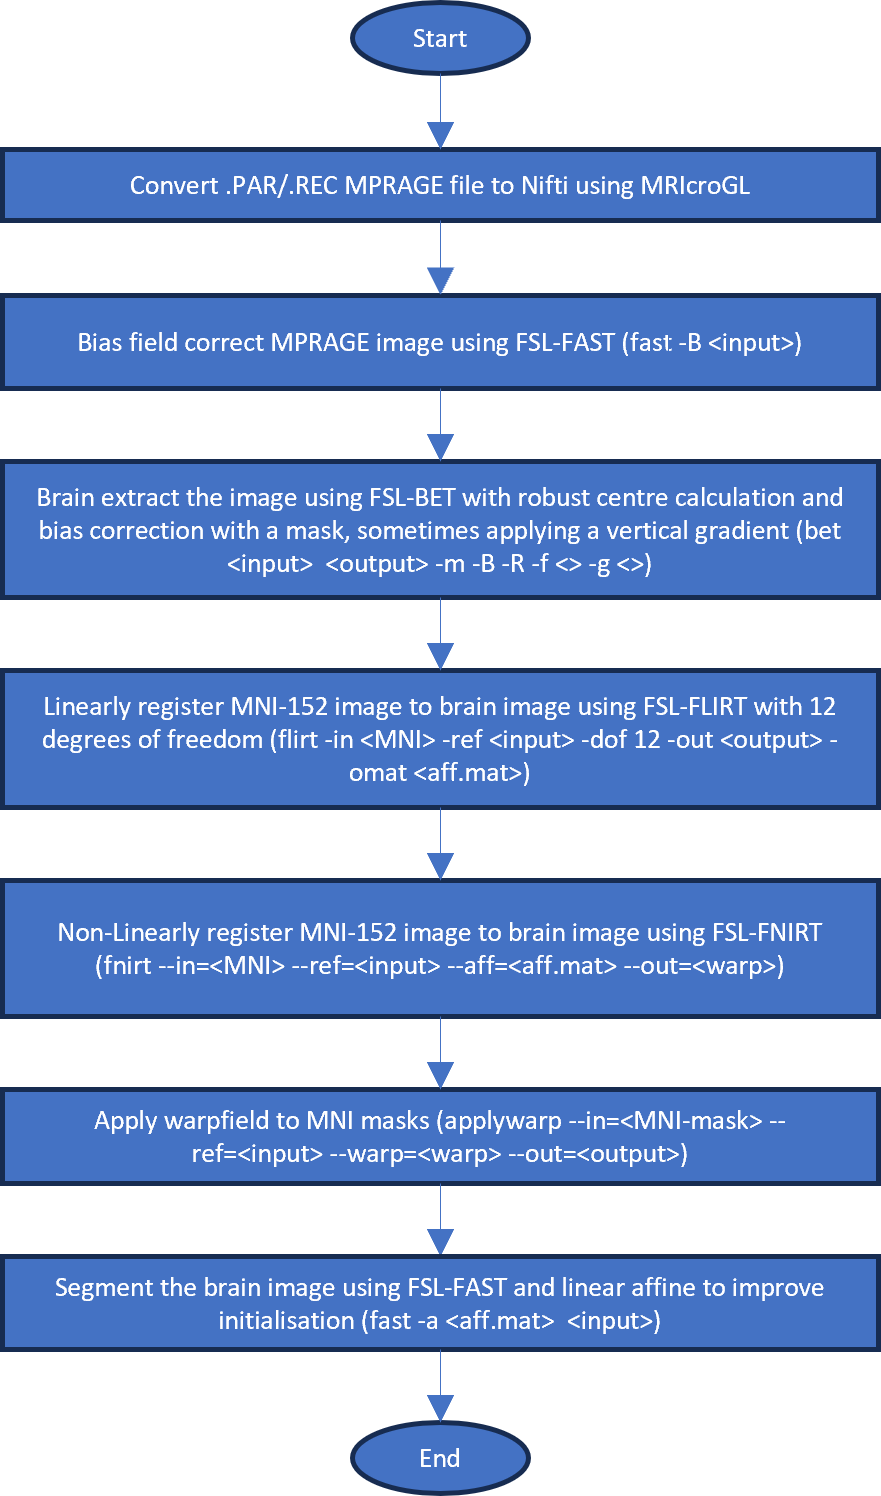
\includegraphics[width = 0.8\textwidth]{Figures/Glucose/Flow_Image.png}
    \caption{\textit{Flowchart outlining the steps used to analyse the $^1$H MPRAGE images and obtain the \ac{ROI} Masks.}}
    \label{fig:Glu:1H_Flow}
\end{figure}

In some of the spectra a noise spike was visible that affected each voxel at the same frequency position. The spike which generally only affected one data point in each spectrum most likely arose from baseline error. To correct this spike the data points immediately either side of corrupted point were averaged together, the spike was replaced with this value. 

Apodisation and smoothing techniques have been shown to affect metabolite quantification in \ac{MRSI} \cite{Goryawala2020EffectsFitting}, which is why it was chosen to not apodise when analysing the data. Low-rank denoising has been shown to be able to use the similarities in temporal/spatial information to denoise, better than for single voxel denoising \cite{Brender2019DynamicHyperpolarization, Goryawala2020EffectsFitting}. Tucker decomposition also known as a \ac{HOSVD} is an extended version of the simpler \ac{SVD}, which is then followed by a low rank approximation. Here only the largest singular values persist, and the rest are replaced with zeros, therefore when reconstructed the data is similar except only the most prominent features persist. This works as a de-noising method as the noise will be represented as smaller singular values and will hence be removed, only leaving the metabolite peaks. This can be performed in either the frequency or the time domain. 

\begin{figure}
    \centering
    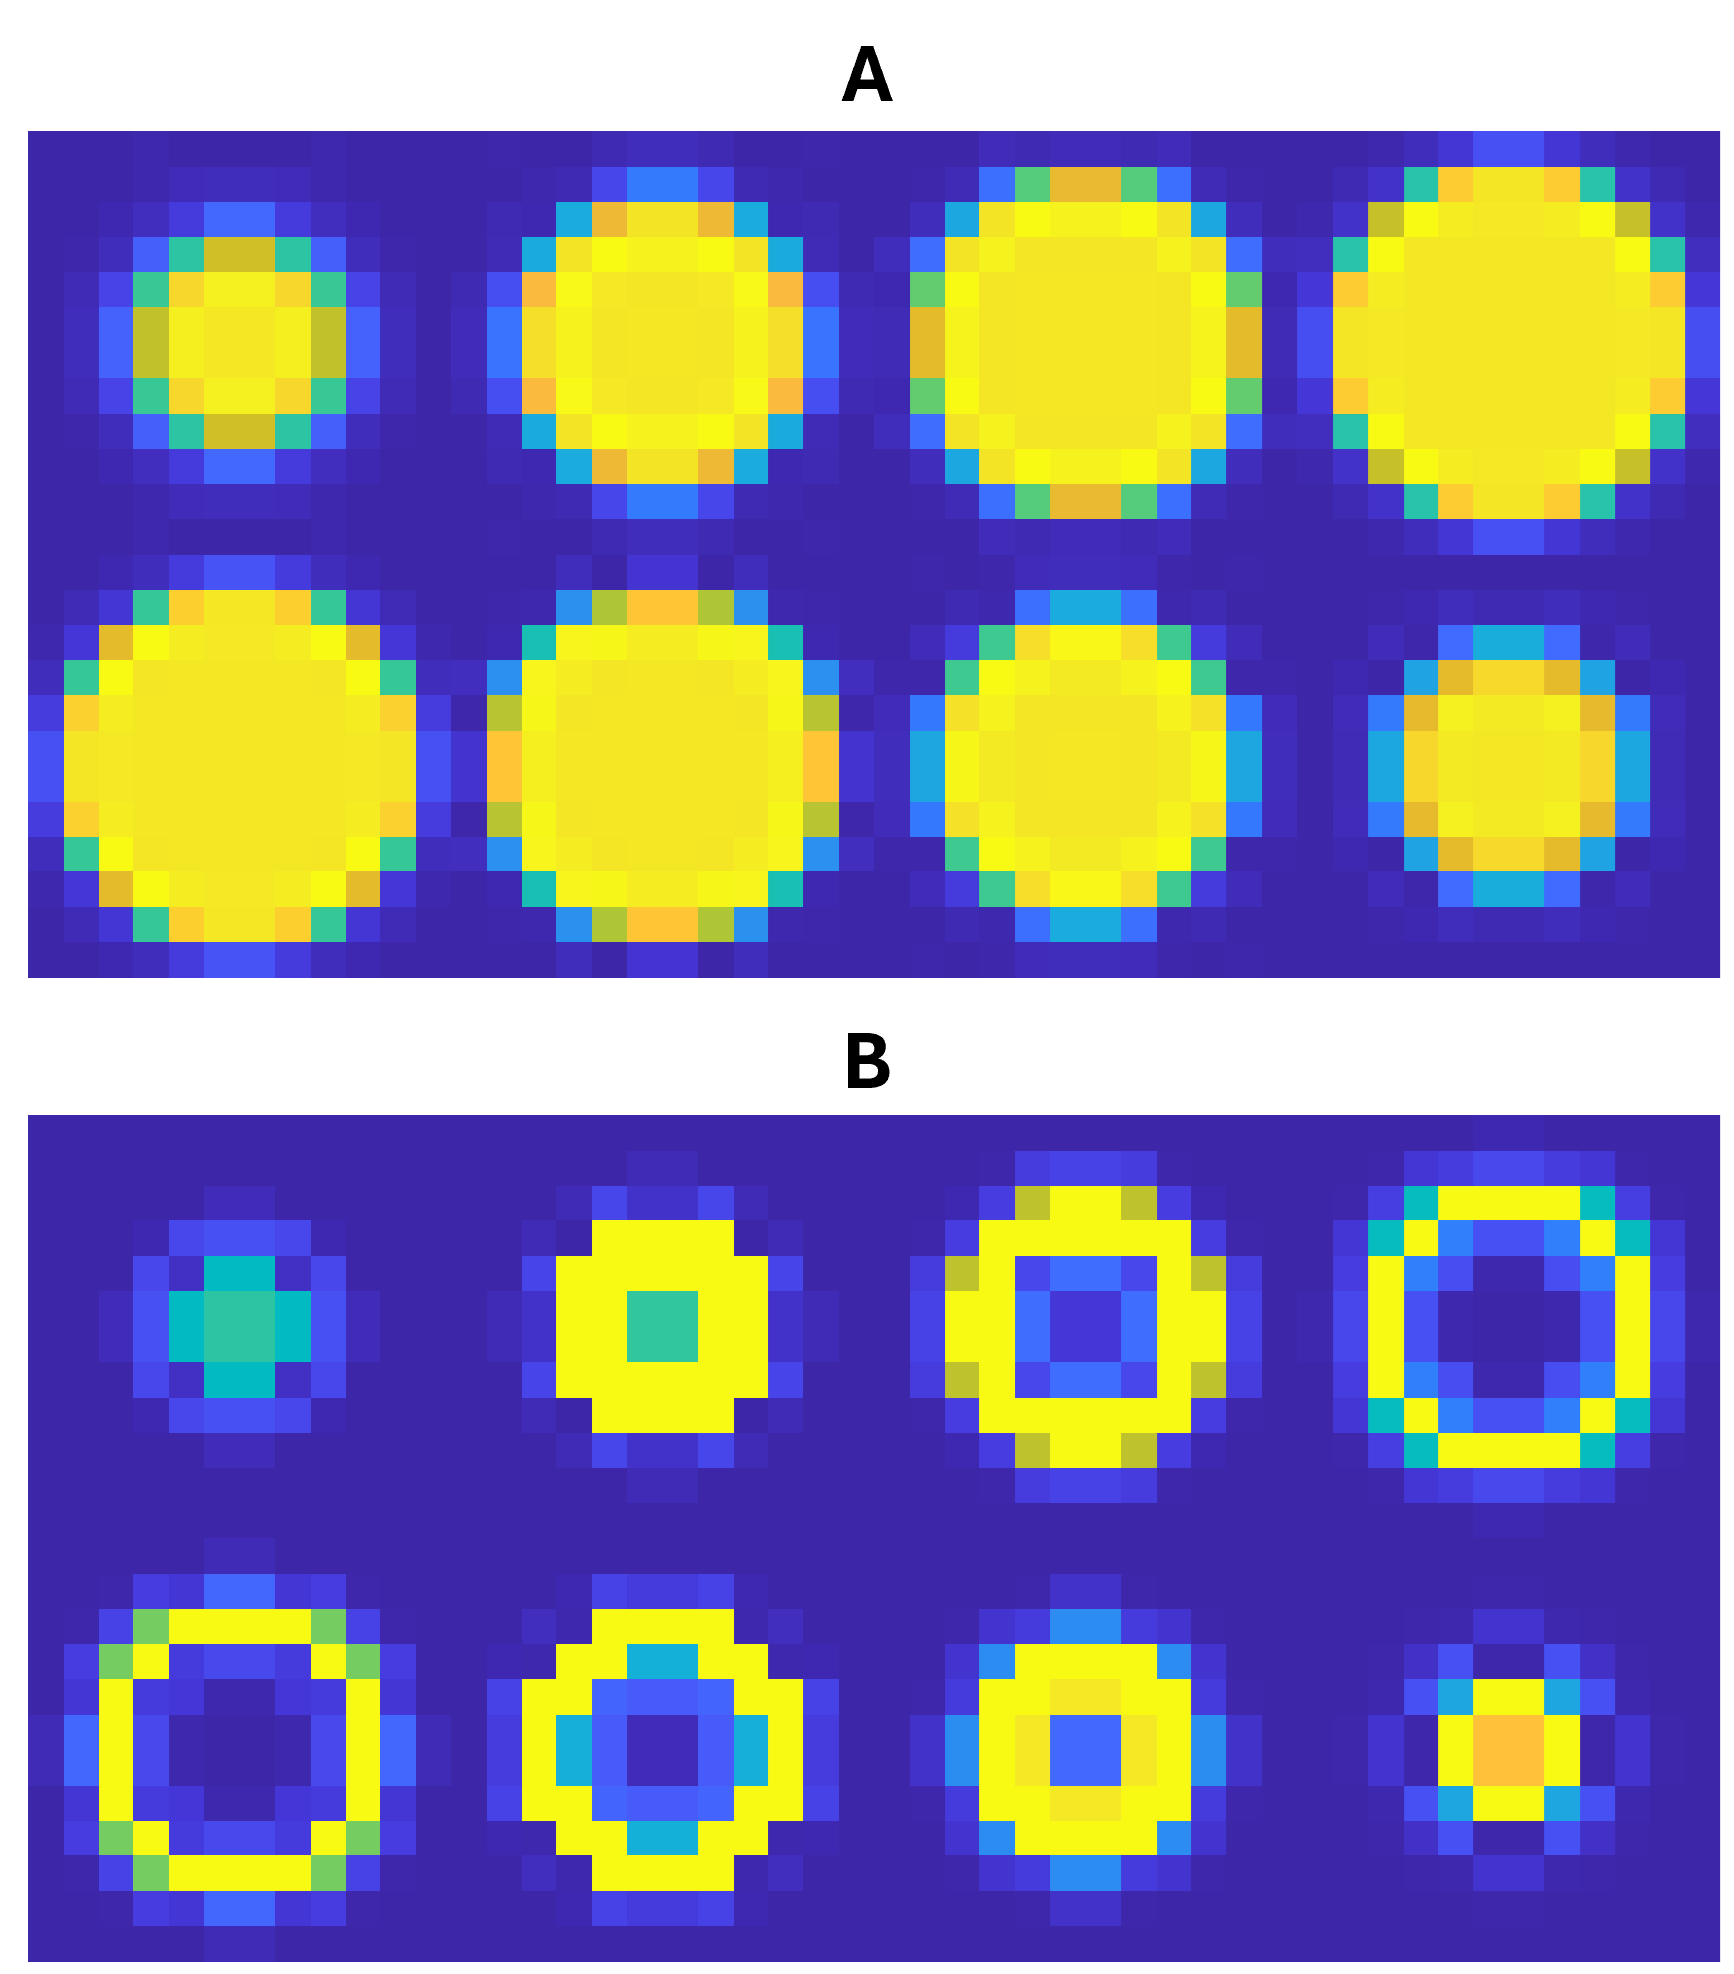
\includegraphics[width = 0.6\textwidth]{Figures/Glucose/Template.png}
    \caption{\textit{3D simulated spherical (A) and hollow-spherical (B) signal distributions used to simulate \ac{DMI} data, for testing different core matrix sizes when de-noising.}}
    \label{fig:Glu:Temp}
\end{figure}

Each \ac{CSI} was denoised in the time-domain using a Tucker decomposition \cite{Bader2007EfficientTensors} with a compression matrix size of [64 6 6 4] (spectral and 3 spatial dimensions). The core matrix size was chosen by simulating 3D \textit{in vivo} $^2$H \ac{CSI} spectra for HDO, glucose and Glx resonances, the amplitude distribution for water and glucose follows a spherical pattern (Fig. \ref{fig:Glu:Temp}A) whilst the amplitude distribution for Glx follows a hollow-sphere (Fig. \ref{fig:Glu:Temp}). Then by varying the core matrix size in a single direction (whilst keeping the others the same) and fitting the spectra, it is possible to compare the signal distribution for each metabolite at each compression size. An example of this can be seen in Fig. \ref{fig:Glu:DeNoise} as the dimensions of the core matrix in the FID sample direction are varied, with the amplitudes for HDO, glucose and Glx being displayed. A choice is then made for the compression in said direction that does not affect the overall distribution for each metabolite whilst still de-noising the data. This is then repeated for each of the other spatial directions until a compression matrix size is obtained. The resulting compression matrix size (relative to total data size) is similar to compression matrix sizes that have been used with \ac{DMI} \cite{vonMorze2021ComparisonT, Kreis2020MeasuringMRI} and C$^{13}$ studies \cite{Brender2019DynamicHyperpolarization}. The visible effect of de-noising using a Tucker decomposition with this core matrix can be seen in Fig. \ref{fig:Glu:DeNoise_spectra}.

\begin{figure}
   \centering
   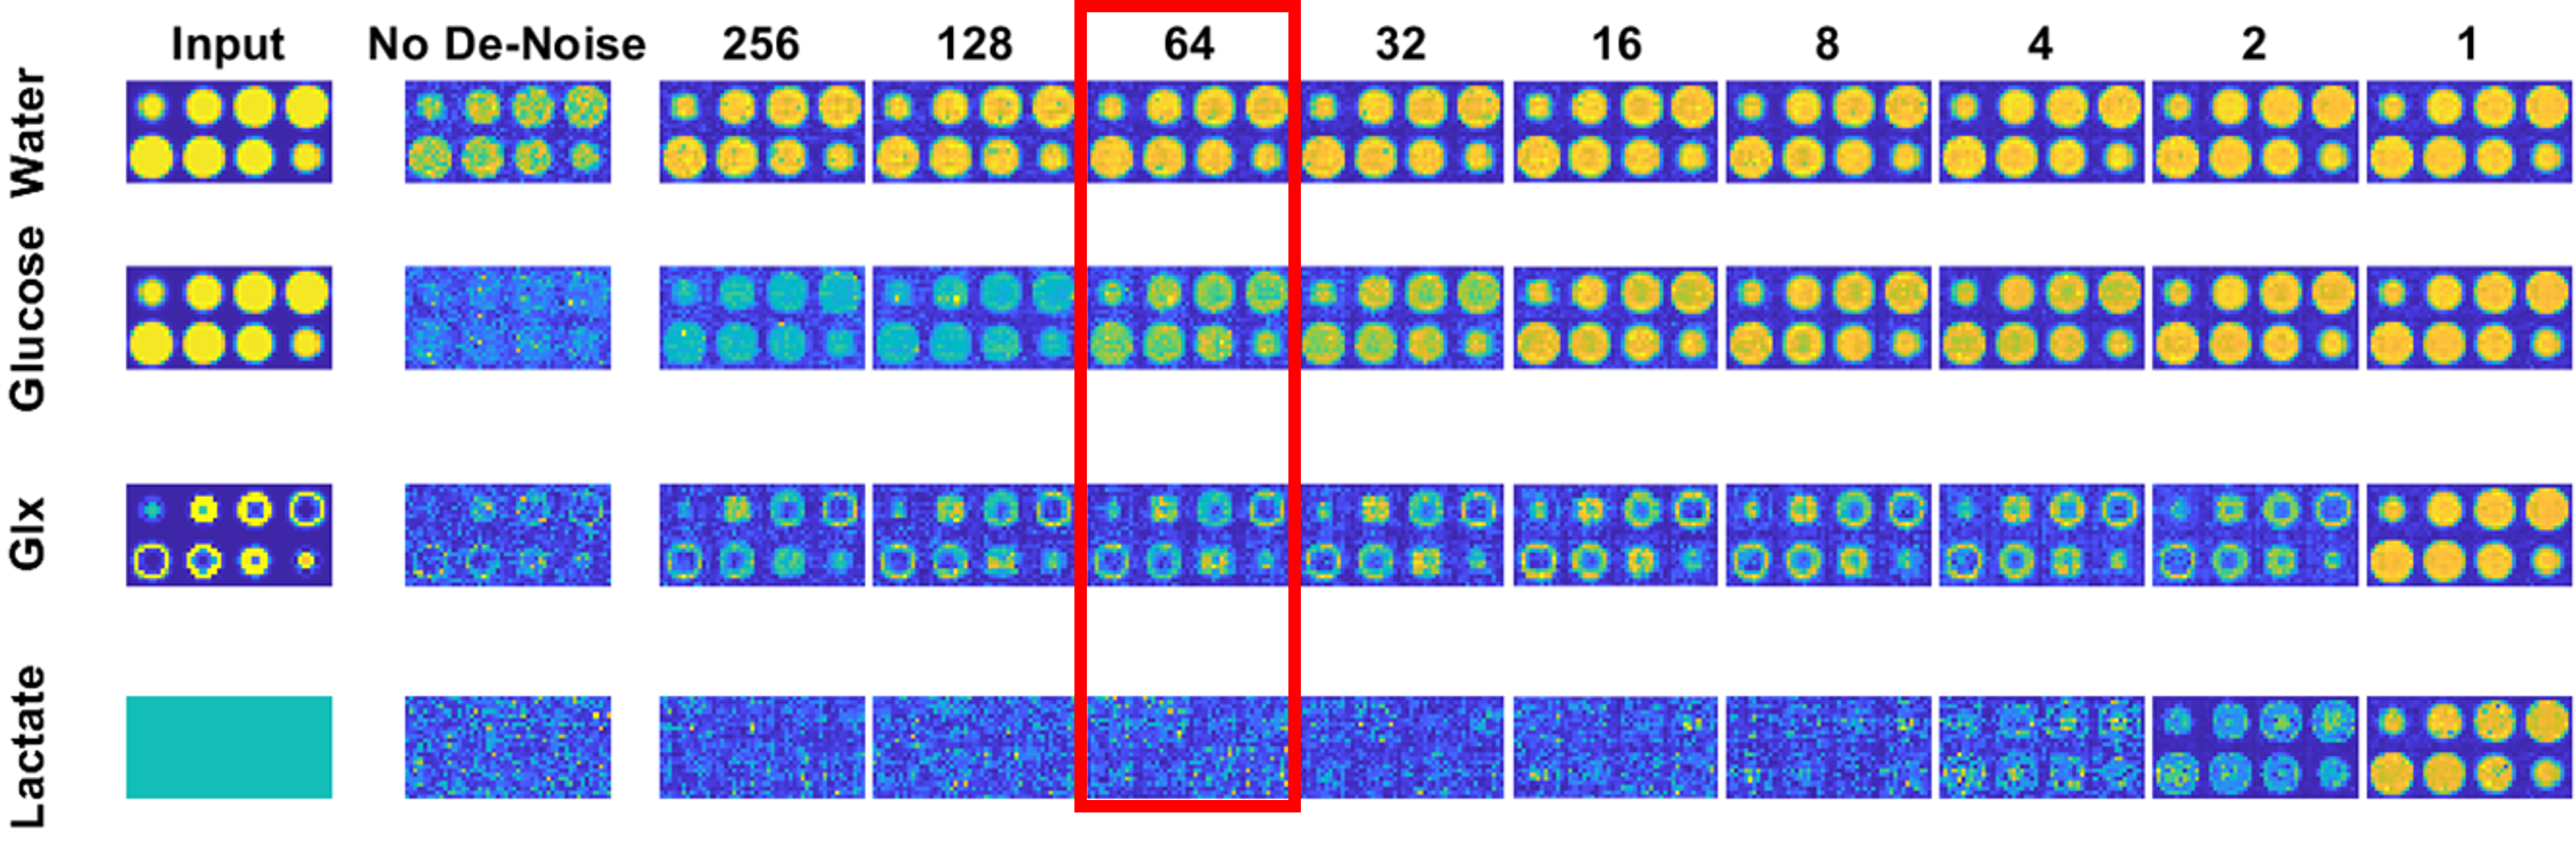
\includegraphics[width = 1\textwidth]{Figures/Glucose/DeNoise_Sim.png}
   \caption{\textit{Ground truth signal distributions for $^2$H water, glucose and Glx (far left) followed by amplitudes obtained from fitting spectra to varying levels of compression in the FID sampling direction. The spatial dimensions are compressed to a core matrix size [6 6 4]. The red box shows the choice of compression for the FID sampling direction.}}
   \label{fig:Glu:DeNoise}
\end{figure}

With low \ac{SNR} datasets it can be possible to bias your data using de-noising, one way to overcome this is to simulate your data and apply varying levels of de-noising which can help choose rank reduction. This was performed with our dataset which helped motivate the choice of rank reduction, which is why de-noising was only applied to each \ac{CSI} and not with a fifth domain of time. It was found that any level of de-noising in this domain smoothed the metabolite change curves, when compared to individual \ac{CSI} de-noising. To avoid biasing the lactate peak (because of its low \ac{SNR}) the simulated data had no true lactate peak present, therefore any presence of lactate above the noise floor in the amplitude maps would indicate too much of a rank reduction. It was found that a rank of eight in the spectral domain and ranks below four in the spatial domain were too small this can be seen in Fig. \ref{fig:Glu:DeNoise}.

\begin{figure}
   \centering
   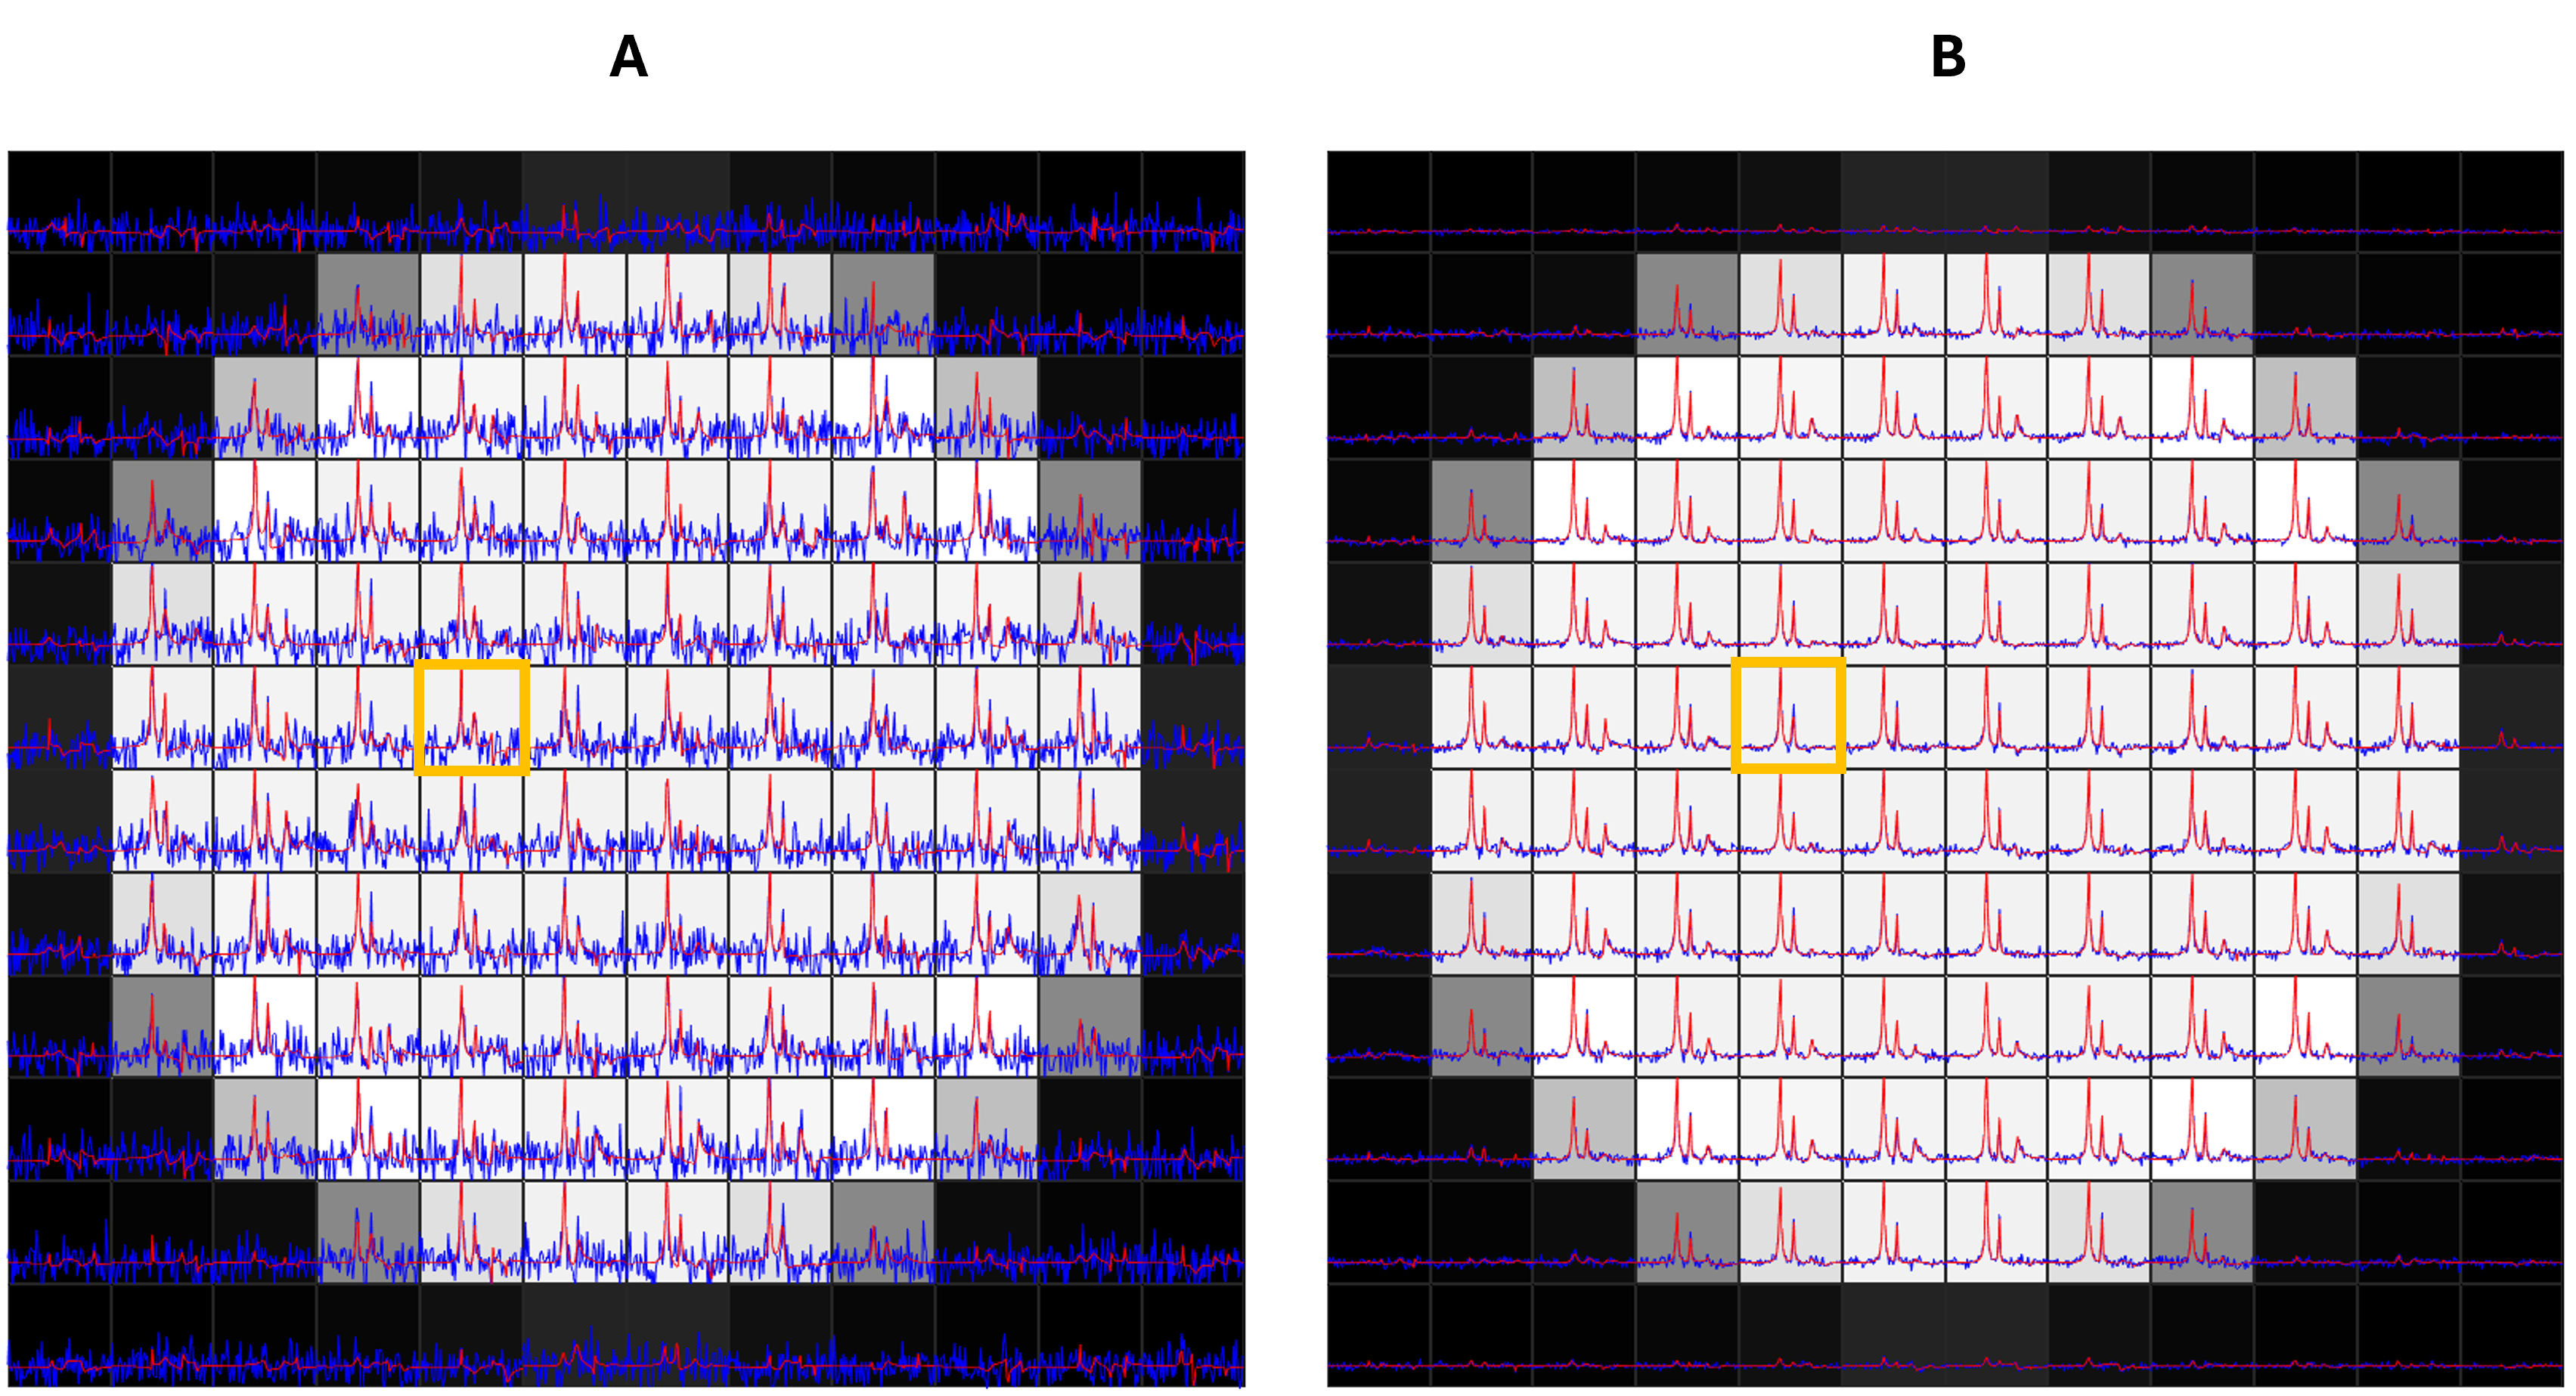
\includegraphics[width = 1\textwidth]{Figures/Glucose/DeNoise_Spectra.png}
   \caption{\textit{\ac{CSI} simulated data (blue) and the corresponding fits (red) for a single slice overlayed onto the sphere from Fig. \ref{fig:Glu:Temp}A. A is the results before de-noising and B is the results after a Tucker decomposition with a core matrix of [64 6 6 4].}}
   \label{fig:Glu:DeNoise_spectra}
\end{figure}

The \ac{FID}s were fitted using an adapted version of the OXSA-\ac{AMARES} MATLAB toolbox \cite{Vanhamme1997ImprovedKnowledge, Purvis2017OXSA:MATLAB}, which requires prior knowledge for each of the metabolites which can be seen in Table \ref{fig:Glu:Prior}. At this point it is important to note that glucose can appear as different anomers, where the chemical composition of the glucose stays the same but the location of the hydroxyl group can swap with the $^1$H on C1. These anomers are called alpha ($\alpha$) and ($\beta$) when dissolved in water 1/3 of glucose will exist in the $\alpha$ form whilst 2/3 will exist in the $\beta$ form. The chemical shifts of glucose (both anomers), Glx, and lactate are assumed to be the same as those of the $^1$H chemical shifts \cite{Govindaraju2000ProtonMetabolites} and were implemented in the fitting as relative shifts to the water peak \cite{Meerwaldt2023InImaging}. Often in previous studies that have used D$_2$-glucose, the spectrum has been fitted as a single peak at 3.8 ppm, since the chemical shift difference between the four resonance lines (two $^2$H labels, two glucose anomers) are usually not discernible due to the relatively broad linewidths and low SNR. However, this is not the case for D$_7$-glucose \cite{Govindaraju2000ProtonMetabolites} which has a larger number of spectral lines and a bigger range of chemical shifts. Therefore, the spectrum needs to be modelled for more accurately, taking into account the contribution from each deuterium label for both anomers. For consistency, this approach was also implemented when analysing the D$_2$-glucose data. The glucose peaks were fitted assuming a common scaling factor; all glucose peaks have the same phase other than the peaks from the C1 position which have a different phase due to large differences in chemical shift. The linewidths of peaks from the same anomer share the same value. For \ac{HDO}, Glx, and lactate, only single components were assumed, with independent amplitudes, phases, and linewidths.

\begin{figure}
    \centering
    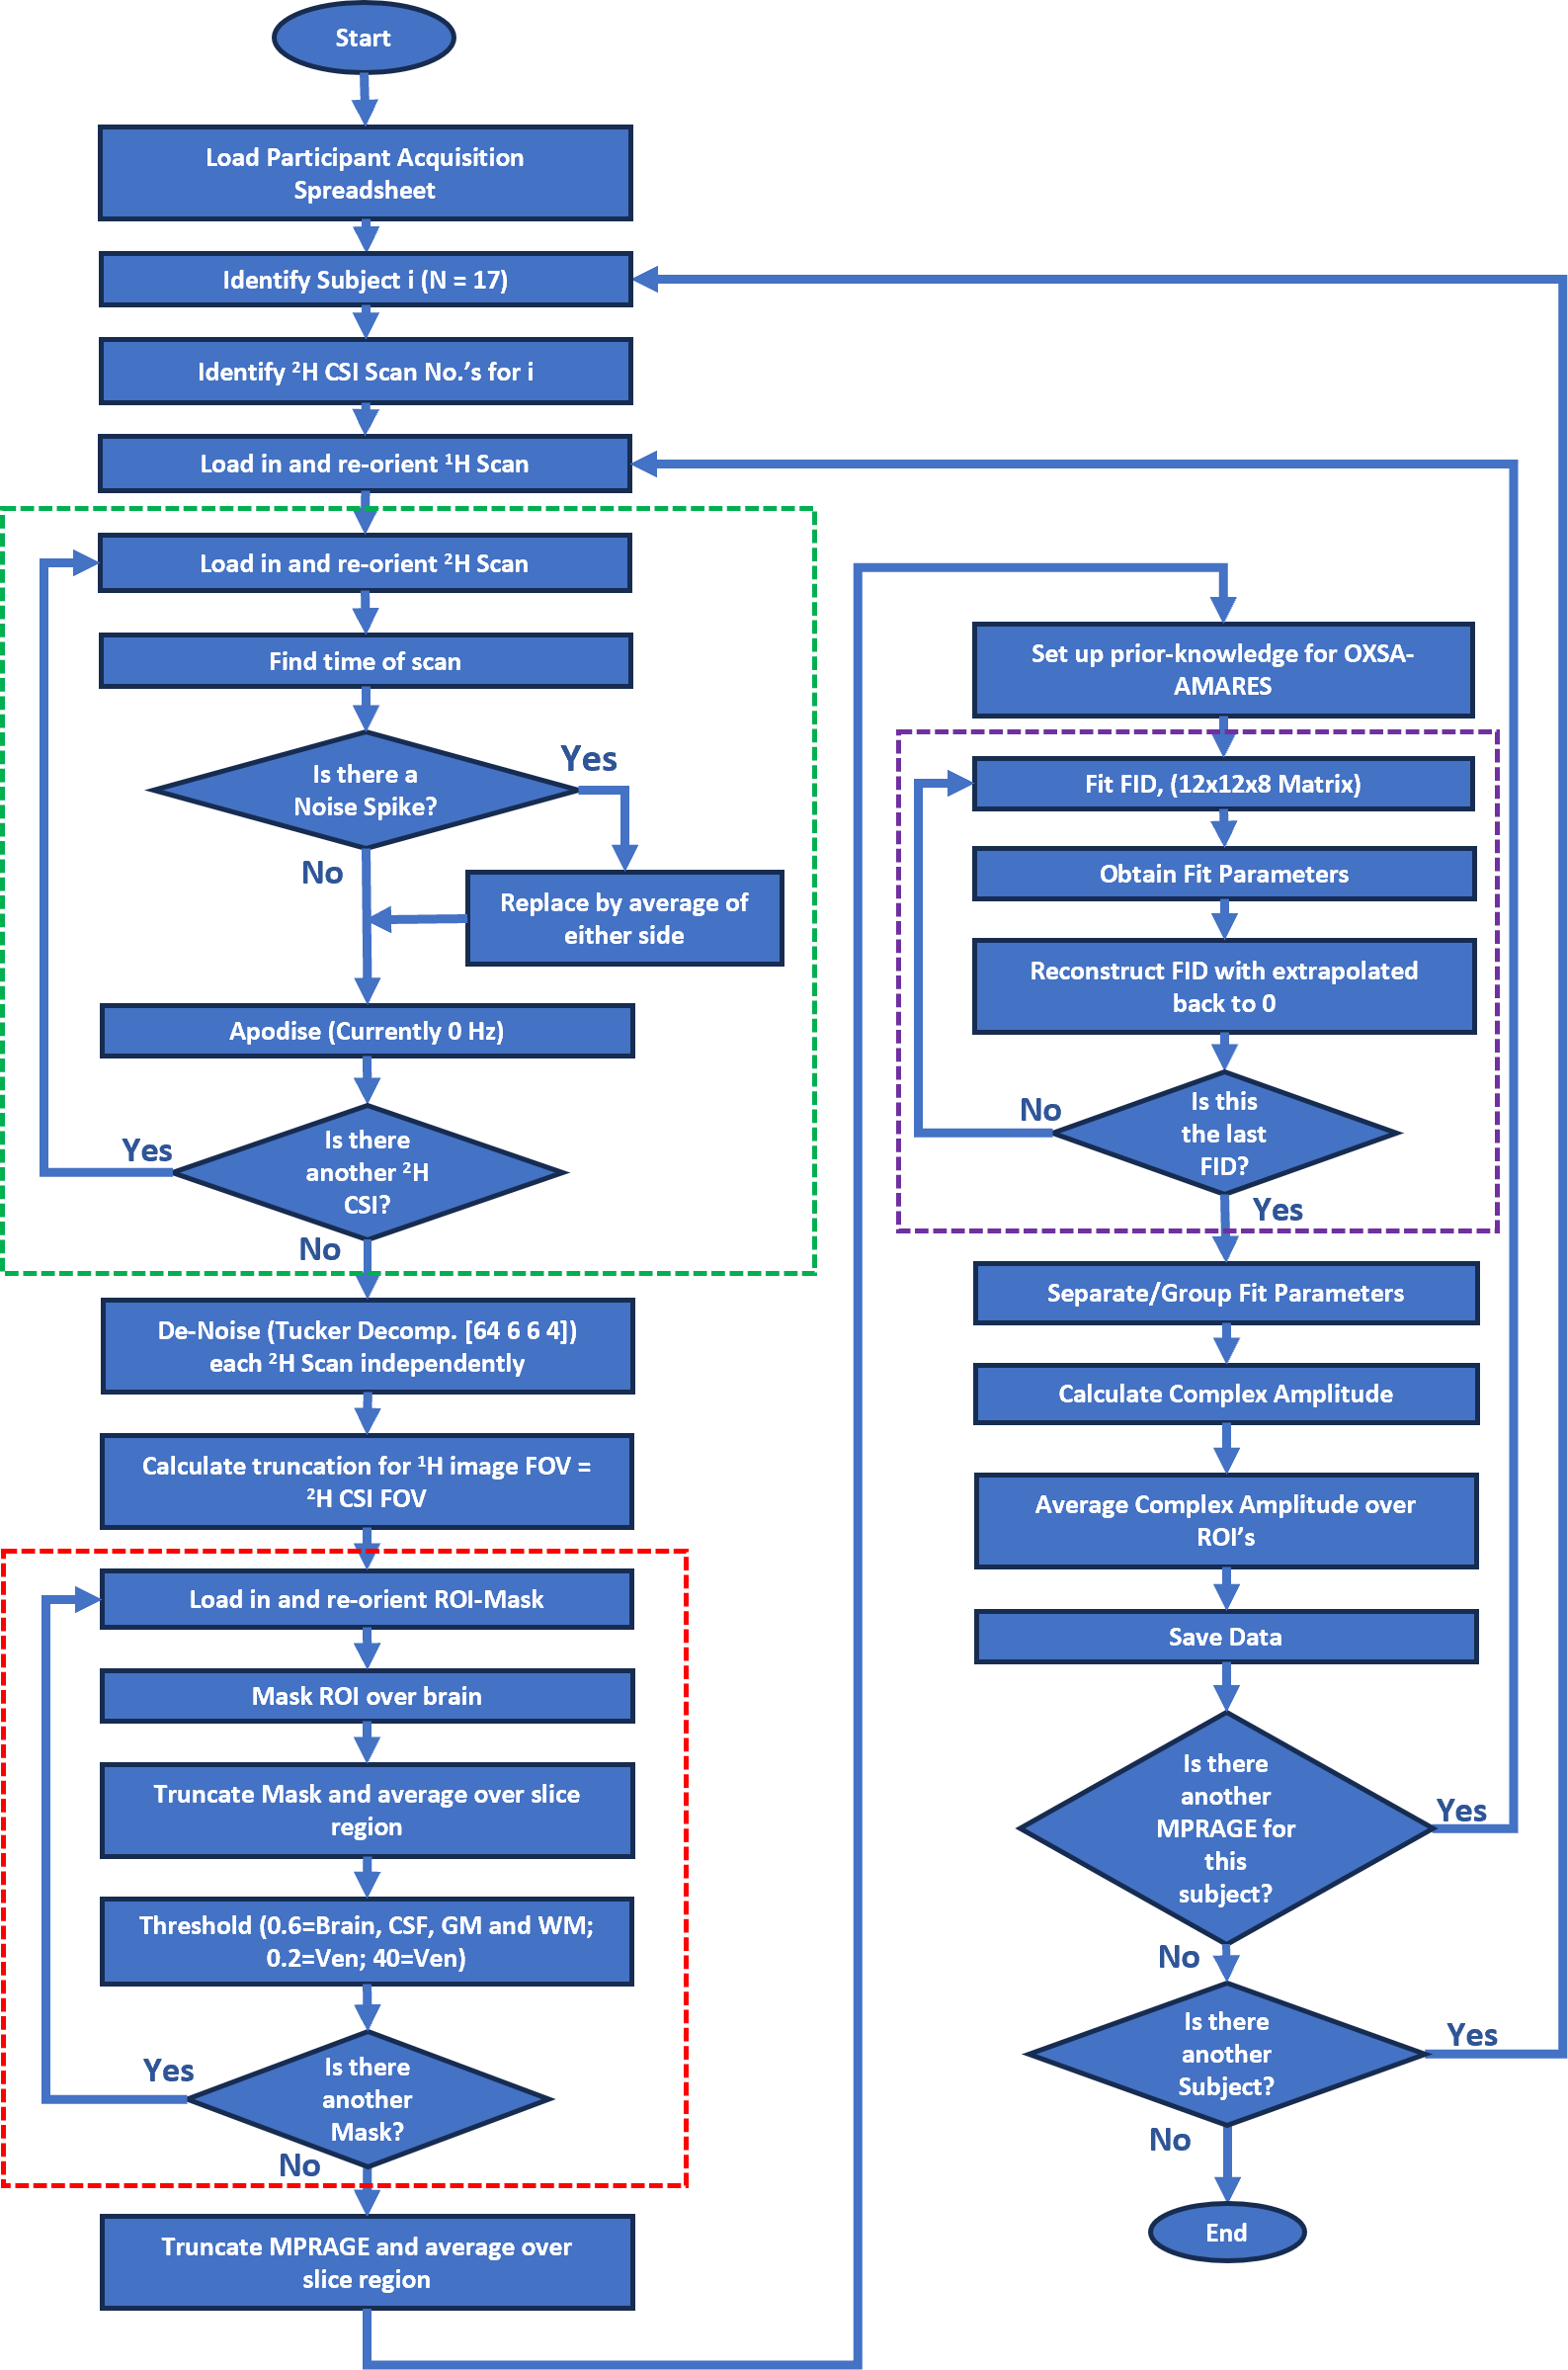
\includegraphics[width = 1\textwidth]{Figures/Glucose/2H_Flow.png}
    \caption{\textit{Flowchart outlining the steps used to analyse the $^2$H \ac{CSI} spectral data (including de-noising). The dotted green box represents the pre-processing steps for the $^2$H data, the dotted red box is the applying of the $^1$H mask and the dotted purple box is the fitting of each spectra.}}
    \label{fig:Glu:2H_Flow}
\end{figure}

One of the obvious difficulties when attempting to fit the D$_7$-glucose data is the extra prior knowledge that has been used, with previous studies fitting the glucose data to as a single peak here the glucose signal is fit as a sum of 14 peaks due to the number of label positions for different anomers $\alpha$ and $\beta$. For completeness the D$_2$-glucose data is fit to 4 peaks for the same reasons, the time increased in the fitting routine between the two fitting routines is approximately 3 times for D$_7$-glucose analysis. The increased complexity of the fitting means it is less likely to accurately fit the \ac{FID} however by narrowing the linewidth constraints and using more accurate initial estimates, as well as lowering the tolerance of the fit (increasing iterations and function evaluations and lowering the function and step tolerance) the fit overlays the data accurately as seen in Figs. \ref{fig:Glu:Select} and \ref{fig:Glu:Avg_Amp}. 

The amplitude and phase values for each metabolite peak at each voxel position were converted to complex amplitudes and interpolated to the same resolution as the \ac{MPRAGE} image. These maps were then averaged over the whole-brain, occipital lobe, 
 and frontal lobe \ac{ROI} (using the binarised segmentation maps) to obtain \ac{ROI}-averaged amplitudes for each metabolite for each \ac{CSI} data-set. This provided amplitude time-courses as a function of time relative to glucose ingestion. These values were then either quantified into concentration values, normalised or corrected for the effect of T$_1$ differences and used as ratios between the two different types of glucose. A flowchart that outlines the steps used to analyse all the $^2$H \ac{CSI} data can be seen in Fig. \ref{fig:Glu:2H_Flow}.

\begin{figure}
    \centering
    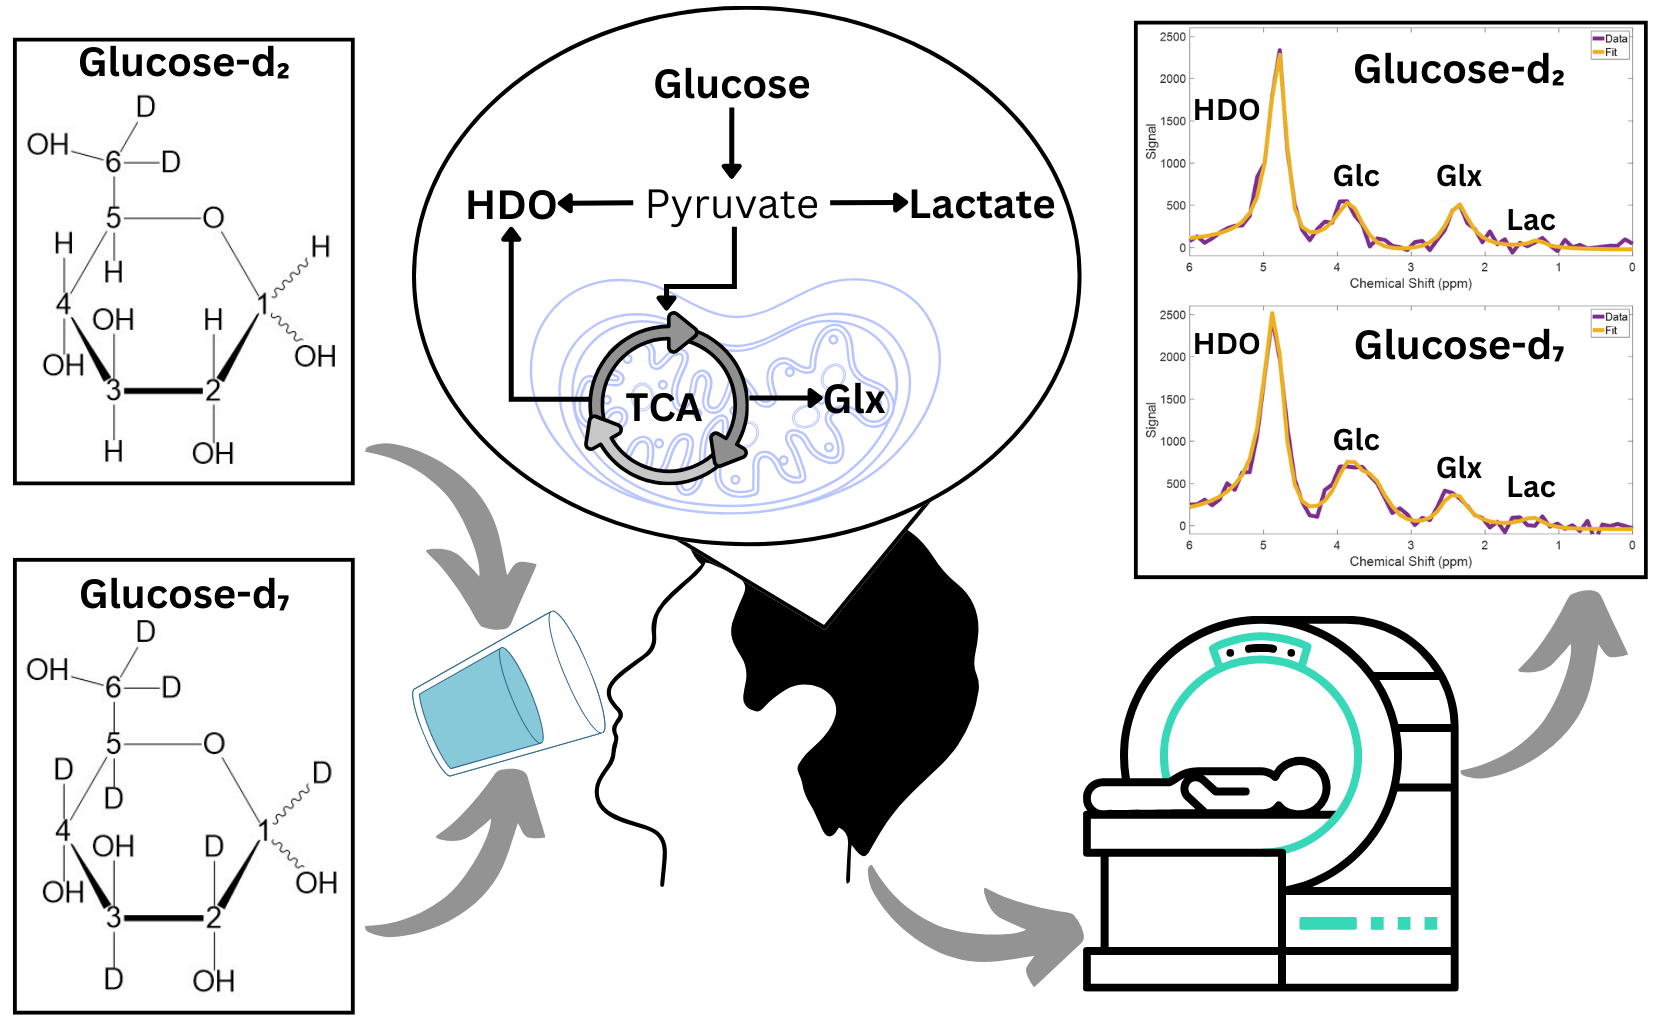
\includegraphics[width = 1\textwidth]{Figures/Glucose/Study_Day.png}
    \caption{\textit{Schematic diagram of the approach used to obtain the $^2$ MRSI data in this study.}}
    \label{fig:Glu:Study_Day}
\end{figure}

\subsection{Concentration calculations}

Concentrations $C^m$ for each metabolite $m$ were determined using the following equation

\begin{equation}
    C^m = \frac{A^m}{kE^mN^m}
    \label{eqn:Glu:Conc}
\end{equation}

where $A^m$ is the FID amplitude of the metabolite, $N^m$ is the number of effective $^2$H labels per metabolite molecule, $E^m$ is the attenuation factor given by

\begin{equation}
    E^m = \frac{1-\exp(-\text{TR}/T_1^m)}{1-\exp(-\text{TR}/T_1^m)\cos{\alpha}}
    \label{eqn:Glu:Atte}
\end{equation}

where T$_1^m$ is the longitudinal relaxation time of the metabolite, TR is the repetition time, $\alpha$ is the flip angle, and $k$ is a scaling constant. This constant, which is found to be \ac{ROI}-dependent, is calculated by using the average \ac{NA} water amplitude within a given \ac{ROI}. This was calculated from the \ac{CSI} data acquired before glucose ingestion assuming an isotopic percentage for deuterium of 0.0156\% \cite{Hagemann1970AbsoluteSMOW}, a concentration of pure water at 55.4 M, a factor of 2 because of the two hydrogen atoms in water, and an estimate of the percentage of water in each \ac{ROI}. Cortical \ac{GM} and \ac{WM} were assumed to be 84\% and 69\% water \cite{Oros-Peusquens2019AImplications}. The occipital and frontal \ac{ROI}s were assumed to be comprised of 40\% \ac{GM} and 60\% \ac{WM}, resulting in a water content of 75\%. The whole brain \ac{ROI} was assumed to be 10\% \ac{CSF}, 36\% \ac{GM}, 54\% \ac{WM}, resulting in 77\% water.

Once $k$ had been estimated for each \ac{ROI}, metabolite concentrations were calculated via Eq. \ref{eqn:Glu:Conc}, with knowledge of the $^2$H label numbers, $N^m$.

The effective number of $^2$H labels depends on whether D$_2$-glucose or D$_7$-glucose was ingested and, for Glx and lactate, also depends onlabel-loss. For D$_2$-glucose, we have assumed the effective number of labels for water, glucose, Glx, and lactate is 1, 2, 1.2, and 1.7, respectively \cite{DeGraaf2021CharacterizationStudies}. For D$_7$-glucose, we have assumed 1, 7, 0.9, and 1.3 (estimated \cite{Funk2017TheGlucose} assuming glutamine and glutamate are present in approximately equal amounts). 

Longitudinal relaxation times for glucose, Glx and lactate were assumed to be 67 ms, 139 ms, and 297 ms, respectively \cite{DeFeyter2018DeuteriumVivo}, independent of \ac{ROI}, number of $^2$H labels, and whether D$_2$-glucose or D$_7$-glucose was the metabolic precursor. For water (\ac{HDO}), the T$_1$ relaxation times were assumed to be 510 ms, 320 ms, and 290 ms for \ac{CSF}, \ac{GM}, and \ac{WM}, respectively \cite{Cocking2023DeuteriumDosing}.

\section{Results}

\begin{figure}
    \centering
    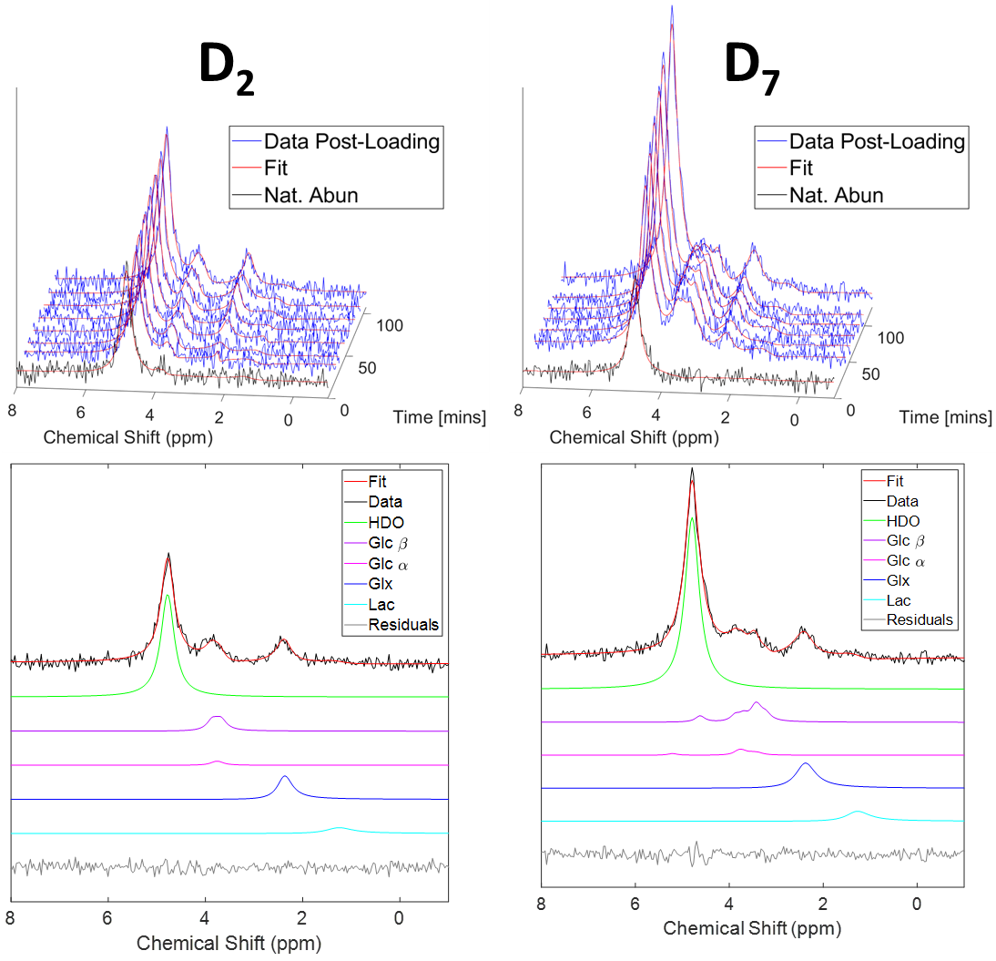
\includegraphics[width = 1\textwidth]{Figures/Glucose/Selective.png}
    \caption{\textit{Stacked selective spectra from a 2-cm-thick slice over the lateral ventricles from individual participants who had ingested D$_2$-glucose (a) or D$_7$-glucose (b). (c-d) Last spectra obtained during scanning with timepoints of $\approx$108 and $\approx$125 minutes, respectively, after glucose ingestion. Corresponding fits are shown for each spectra, along with separated contributions from each metabolite and the residuals after fitting.}}
    \label{fig:Glu:Select}
\end{figure}

Figure \ref{fig:Glu:Select} shows spectra acquired from a 2-cm thick axial slice positioned over the lateral ventricles in two participants before and after ingesting D$_2$- or D$_7$-glucose. The spectra are displayed with the same signal intensity axis scale so that the greater amplitudes of the signals following D$_7$-glucose ingestion are evident, especially for the \ac{HDO}. Single spectra obtained $\approx$108 minutes and $\approx$125 minutes after D$_2$-glucose and D$_7$-glucose ingestion respectively are also shown, along with the fits, and the individual contributions to the fit from \ac{HDO}, glucose (each anomer), Glx and lactate. The glucose signals include contributions from each anomer ($\alpha$ and $\beta$) and each label position. D$_7$-glucose produces a broader peak, centred around 3.7 ppm, compared to D$_2$-glucose, and there are additional resonances at $\approx$5.2 and $\approx$4.6 ppm from the C1 deuterium of the two anomers in the D$_7$-glucose spectra. The \ac{HDO}, Glx and lactate signals show no obvious differences in linewidths and chemical shift position between glucose isotopologues or times after glucose ingestion. No obvious peak is visible above the noise floor in the residual spectrum, indicating the fitting performed well, notably this is true for the more intricate glucose signal from D$_7$-glucose.

\begin{figure}
    \centering
    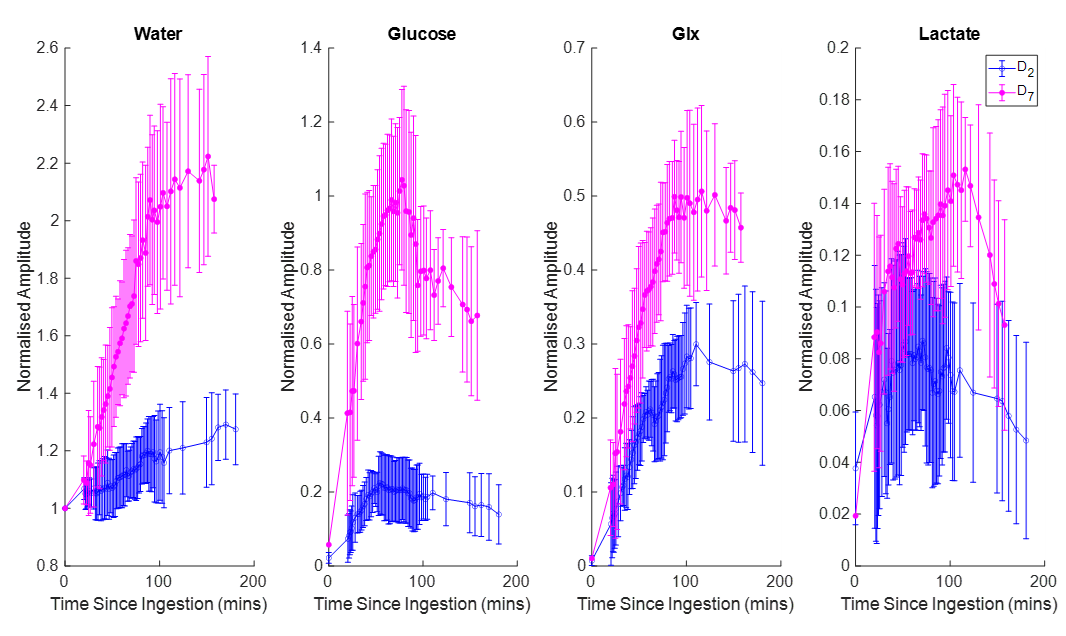
\includegraphics[width = 1\textwidth]{Figures/Glucose/Bulk_Time.png}
    \caption{\textit{Average time-courses of normalised metabolite signals taken from the slice selective spectra from participants who ingested D$_2$-glucose (blue) and D$_7$-glucose (pink). A moving average which over the nearest points in time equal to the number of participants, with error bars representing the moving standard deviation.}}
    \label{fig:Glu:Select_Time}
\end{figure}

The overall time-courses obtained from analysing all the slice-selective spectra for all participants who ingested D$_2$-glucose and D$_7$-glucose can be seen in Fig. \ref{fig:Glu:Select_Time}. It is important to note that no line broadening/apodisation or de-noising technique has been applied here prior to fitting. The data is normalised to the \ac{NA} HDO signal obtained prior to ingestion. The increase in signal for each metabolite can be seen here. The reported lactate signal here could arise from lipids as it has the same chemical shift, however it is not expected to see any $^2$H incorporation into lipids from the labelled glucose.  

\begin{figure}
    \centering
    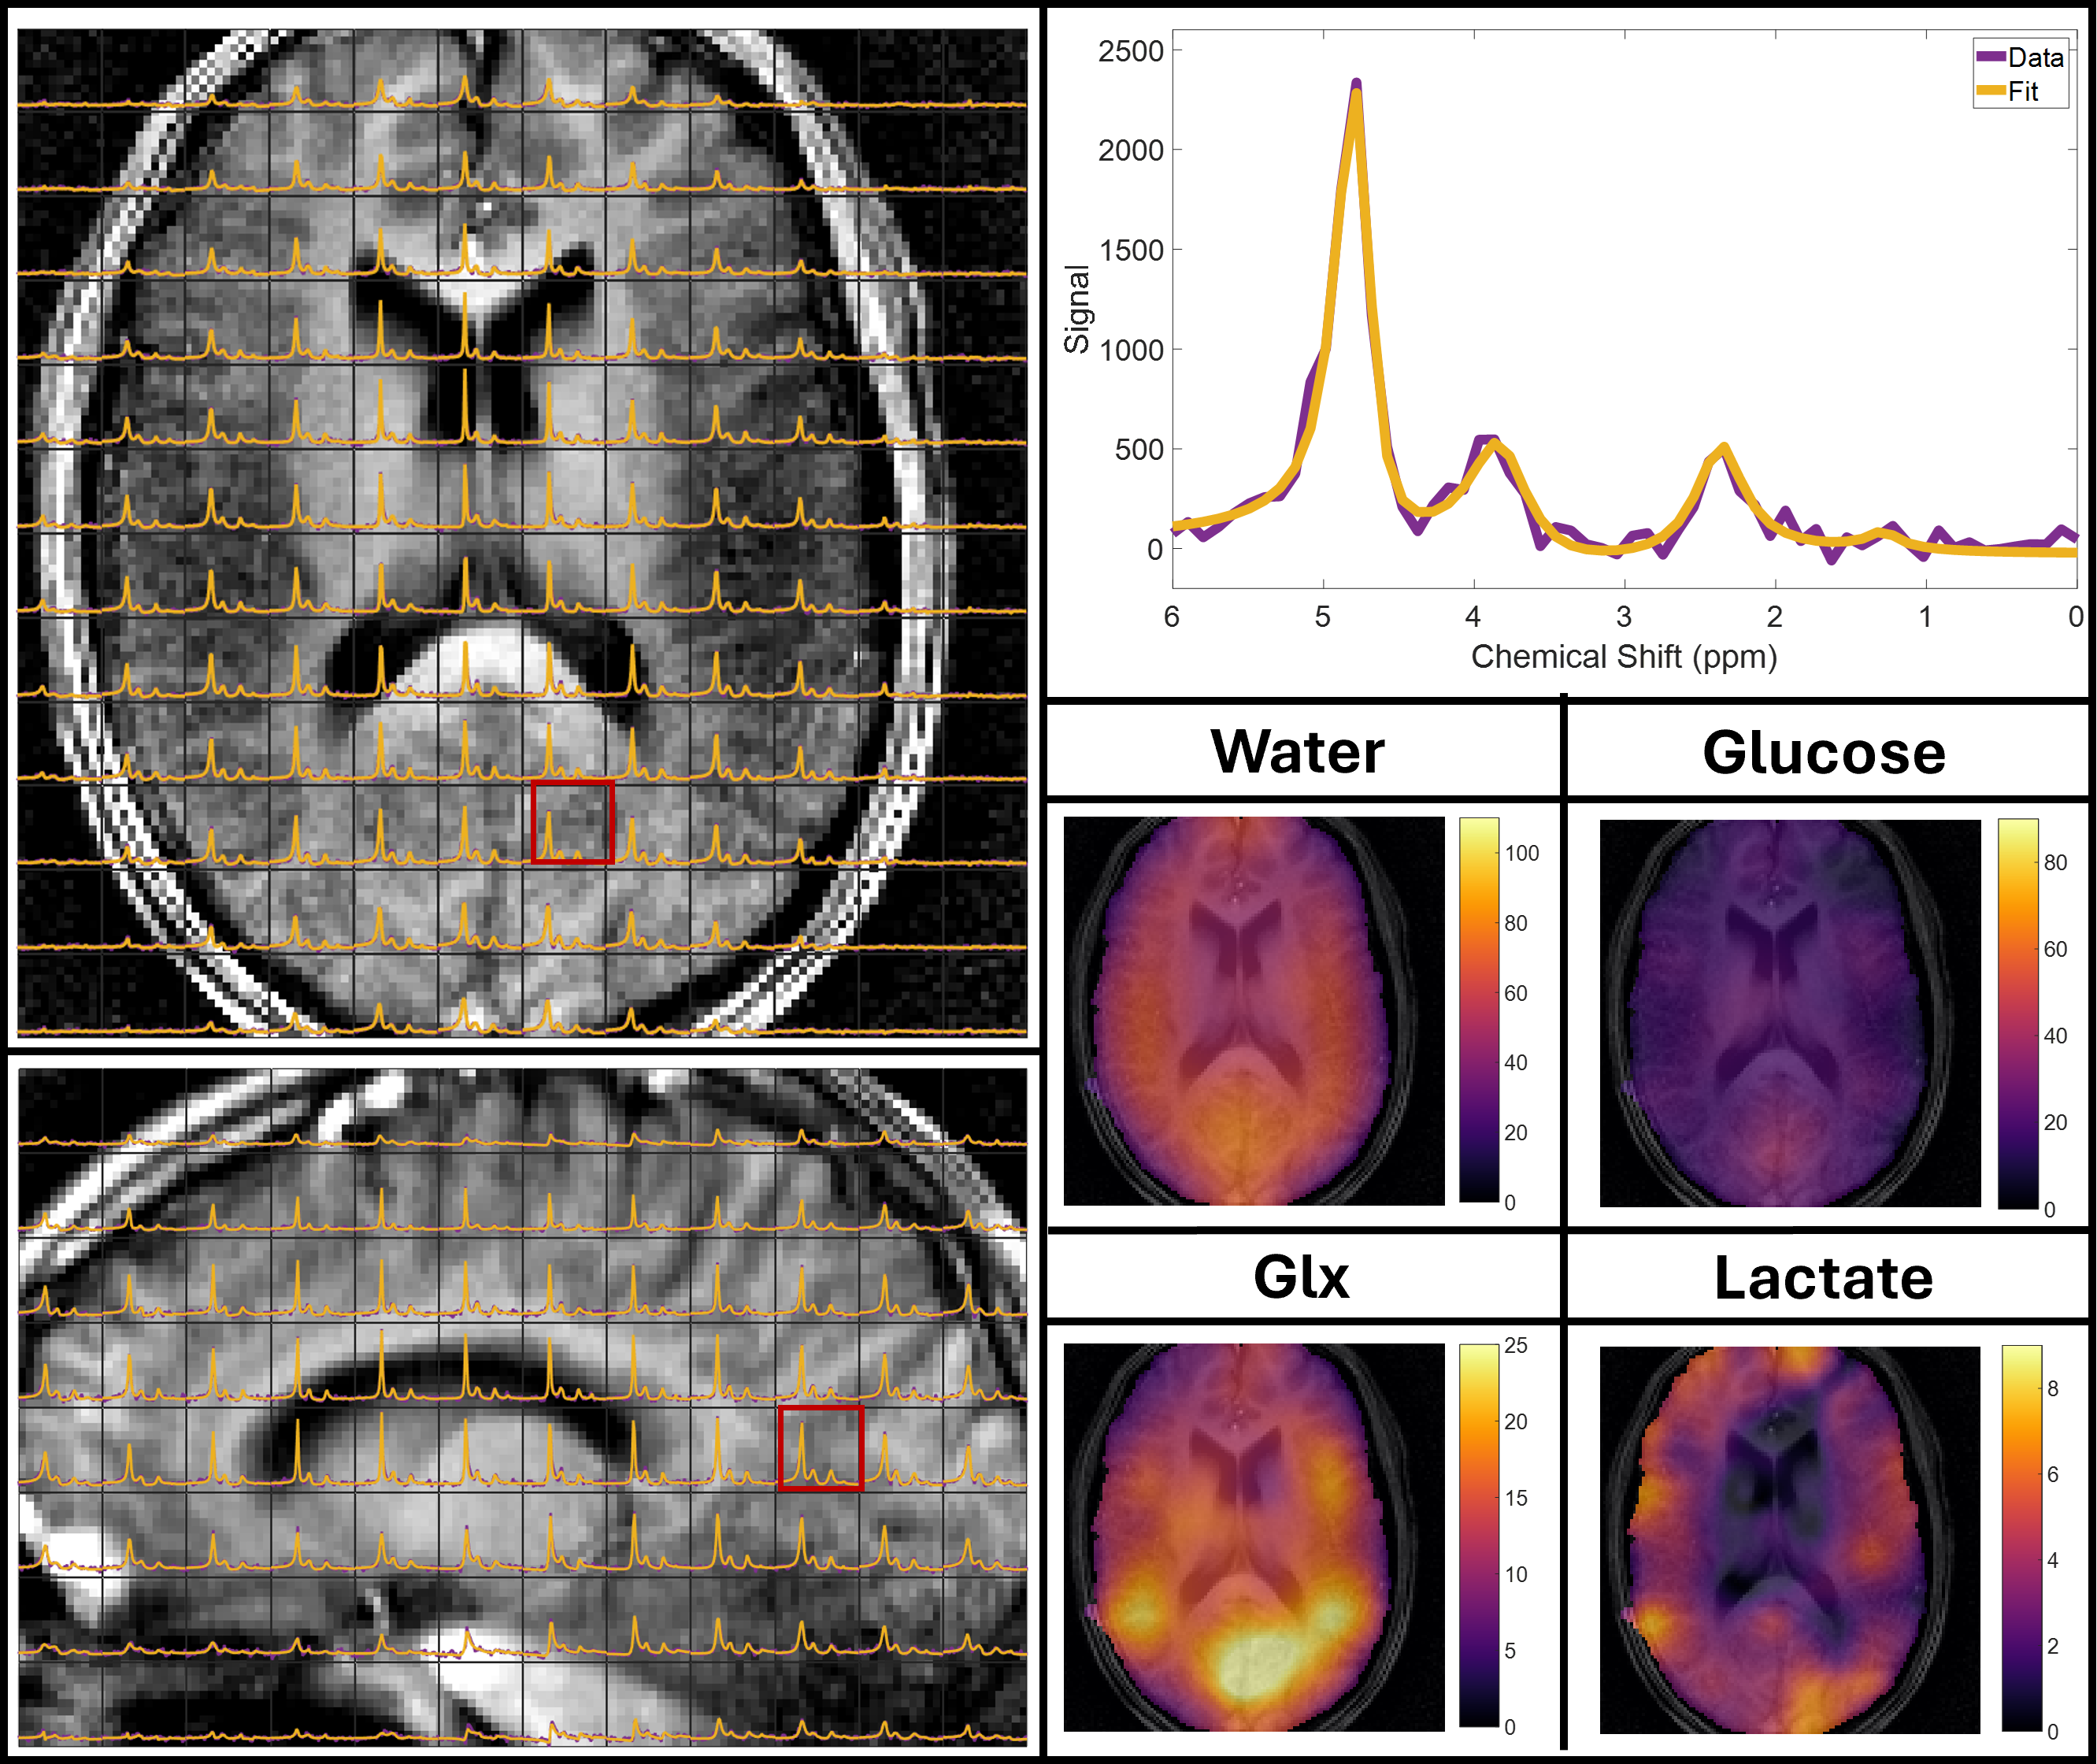
\includegraphics[width = 1\textwidth]{Figures/Glucose/D2_CSI.png}
    \caption{\textit{Axial and sagittal slices of the 3D \ac{CSI} data set (\ac{FOV}: 180x180x120 mm$^3$, 15 mm isotropic resolution) from a participant after ingestion of D$_2$-glucose. Spectra were averaged over six scans and then denoised using a Tucker decomposition and are overlaid on the corresponding slice of the \ac{MPRAGE} image acquired after ingestion. Experimental data (purple) and fits (yellow) are shown for each voxel. The spectra from the highlighted voxels are shown in detail in the lower plots. Amplitude maps for each metabolite are shown below, with the colour axis being shared with Fig. \ref{fig:Glu:D7_CSI}.}}
    \label{fig:Glu:D2_CSI}
\end{figure}

\begin{figure}
    \centering
    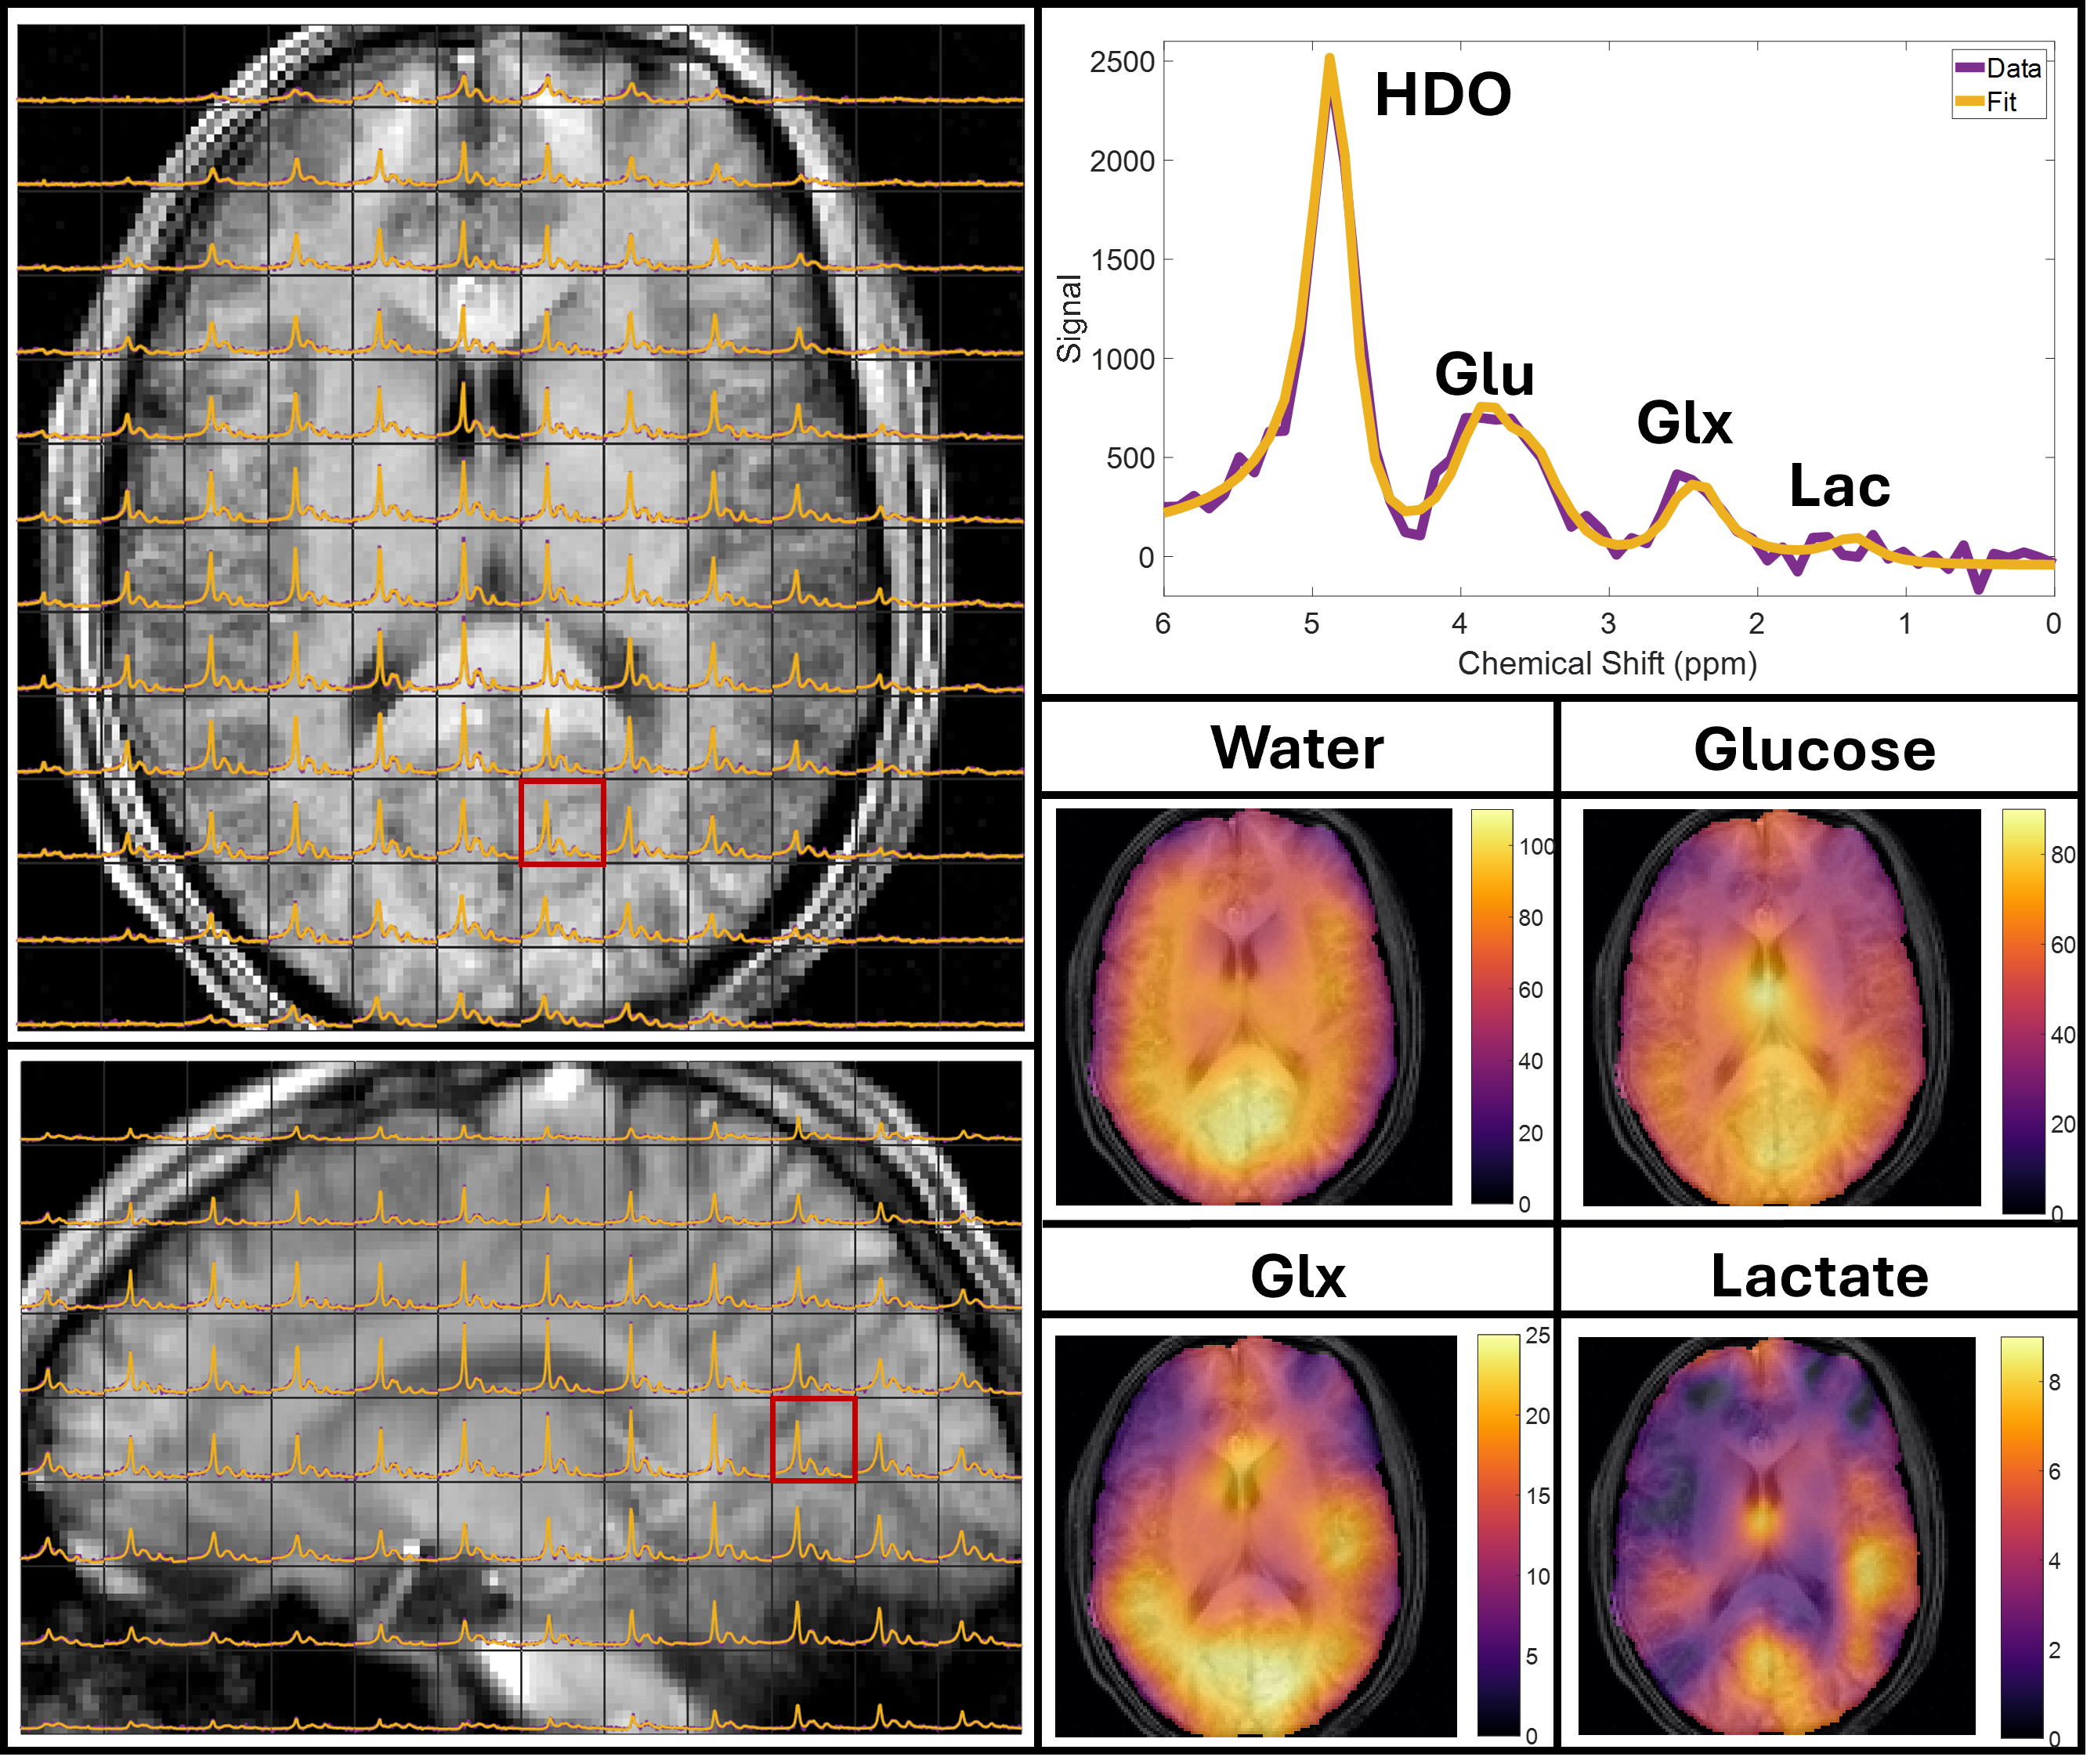
\includegraphics[width = 1\textwidth]{Figures/Glucose/D7_CSI.png}
    \caption{\textit{Axial and sagittal slices of the 3D \ac{CSI} data set (\ac{FOV}: 180x180x120 mm$^3$, 15 mm isotropic resolution) from a participant after ingestion of D$_7$-glucose. Spectra were averaged over six scans and then denoised using a Tucker decomposition and are overlaid on the corresponding slice of the \ac{MPRAGE} image acquired after ingestion. Experimental data (purple) and fits (yellow) are shown for each voxel. The spectra from the highlighted voxels are shown in detail in the lower plots. Amplitude maps for each metabolite are shown below, with the colour axis being shared with Fig. \ref{fig:Glu:D2_CSI}.}}
    \label{fig:Glu:D7_CSI}
\end{figure}

Axial and sagittal slices from denoised 3D \ac{CSI} data, averaged over six scans are shown in Figs. \ref{fig:Glu:D2_CSI} and \ref{fig:Glu:D7_CSI} for two participants, with the overall fits to each voxel. The spectral data is overlaid on the bias-field-corrected $^1$H \ac{MPRAGE} image. Spectra and corresponding fits from the highlighted voxels (red) in both the axial and sagittal view are also shown, the spectra are similar in appearance to those displayed in the slice-selective spectra of Fig. \ref{fig:Glu:Select}. Interpolated and overlaid, axial, amplitude maps of each of the metabolites of one slice are shown in Figs. \ref{fig:Glu:D2_CSI} and \ref{fig:Glu:D7_CSI} after ingestion of D$_2$-glucose and D$_7$-glucose for two participants. The \ac{FID} amplitude values, for each metabolite, are obtained from fitting the averaged \ac{CSI} data after denoising using OXSA-AMARES \cite{Vanhamme1997ImprovedKnowledge, Purvis2017OXSA:MATLAB}.

\begin{figure}
    \centering
    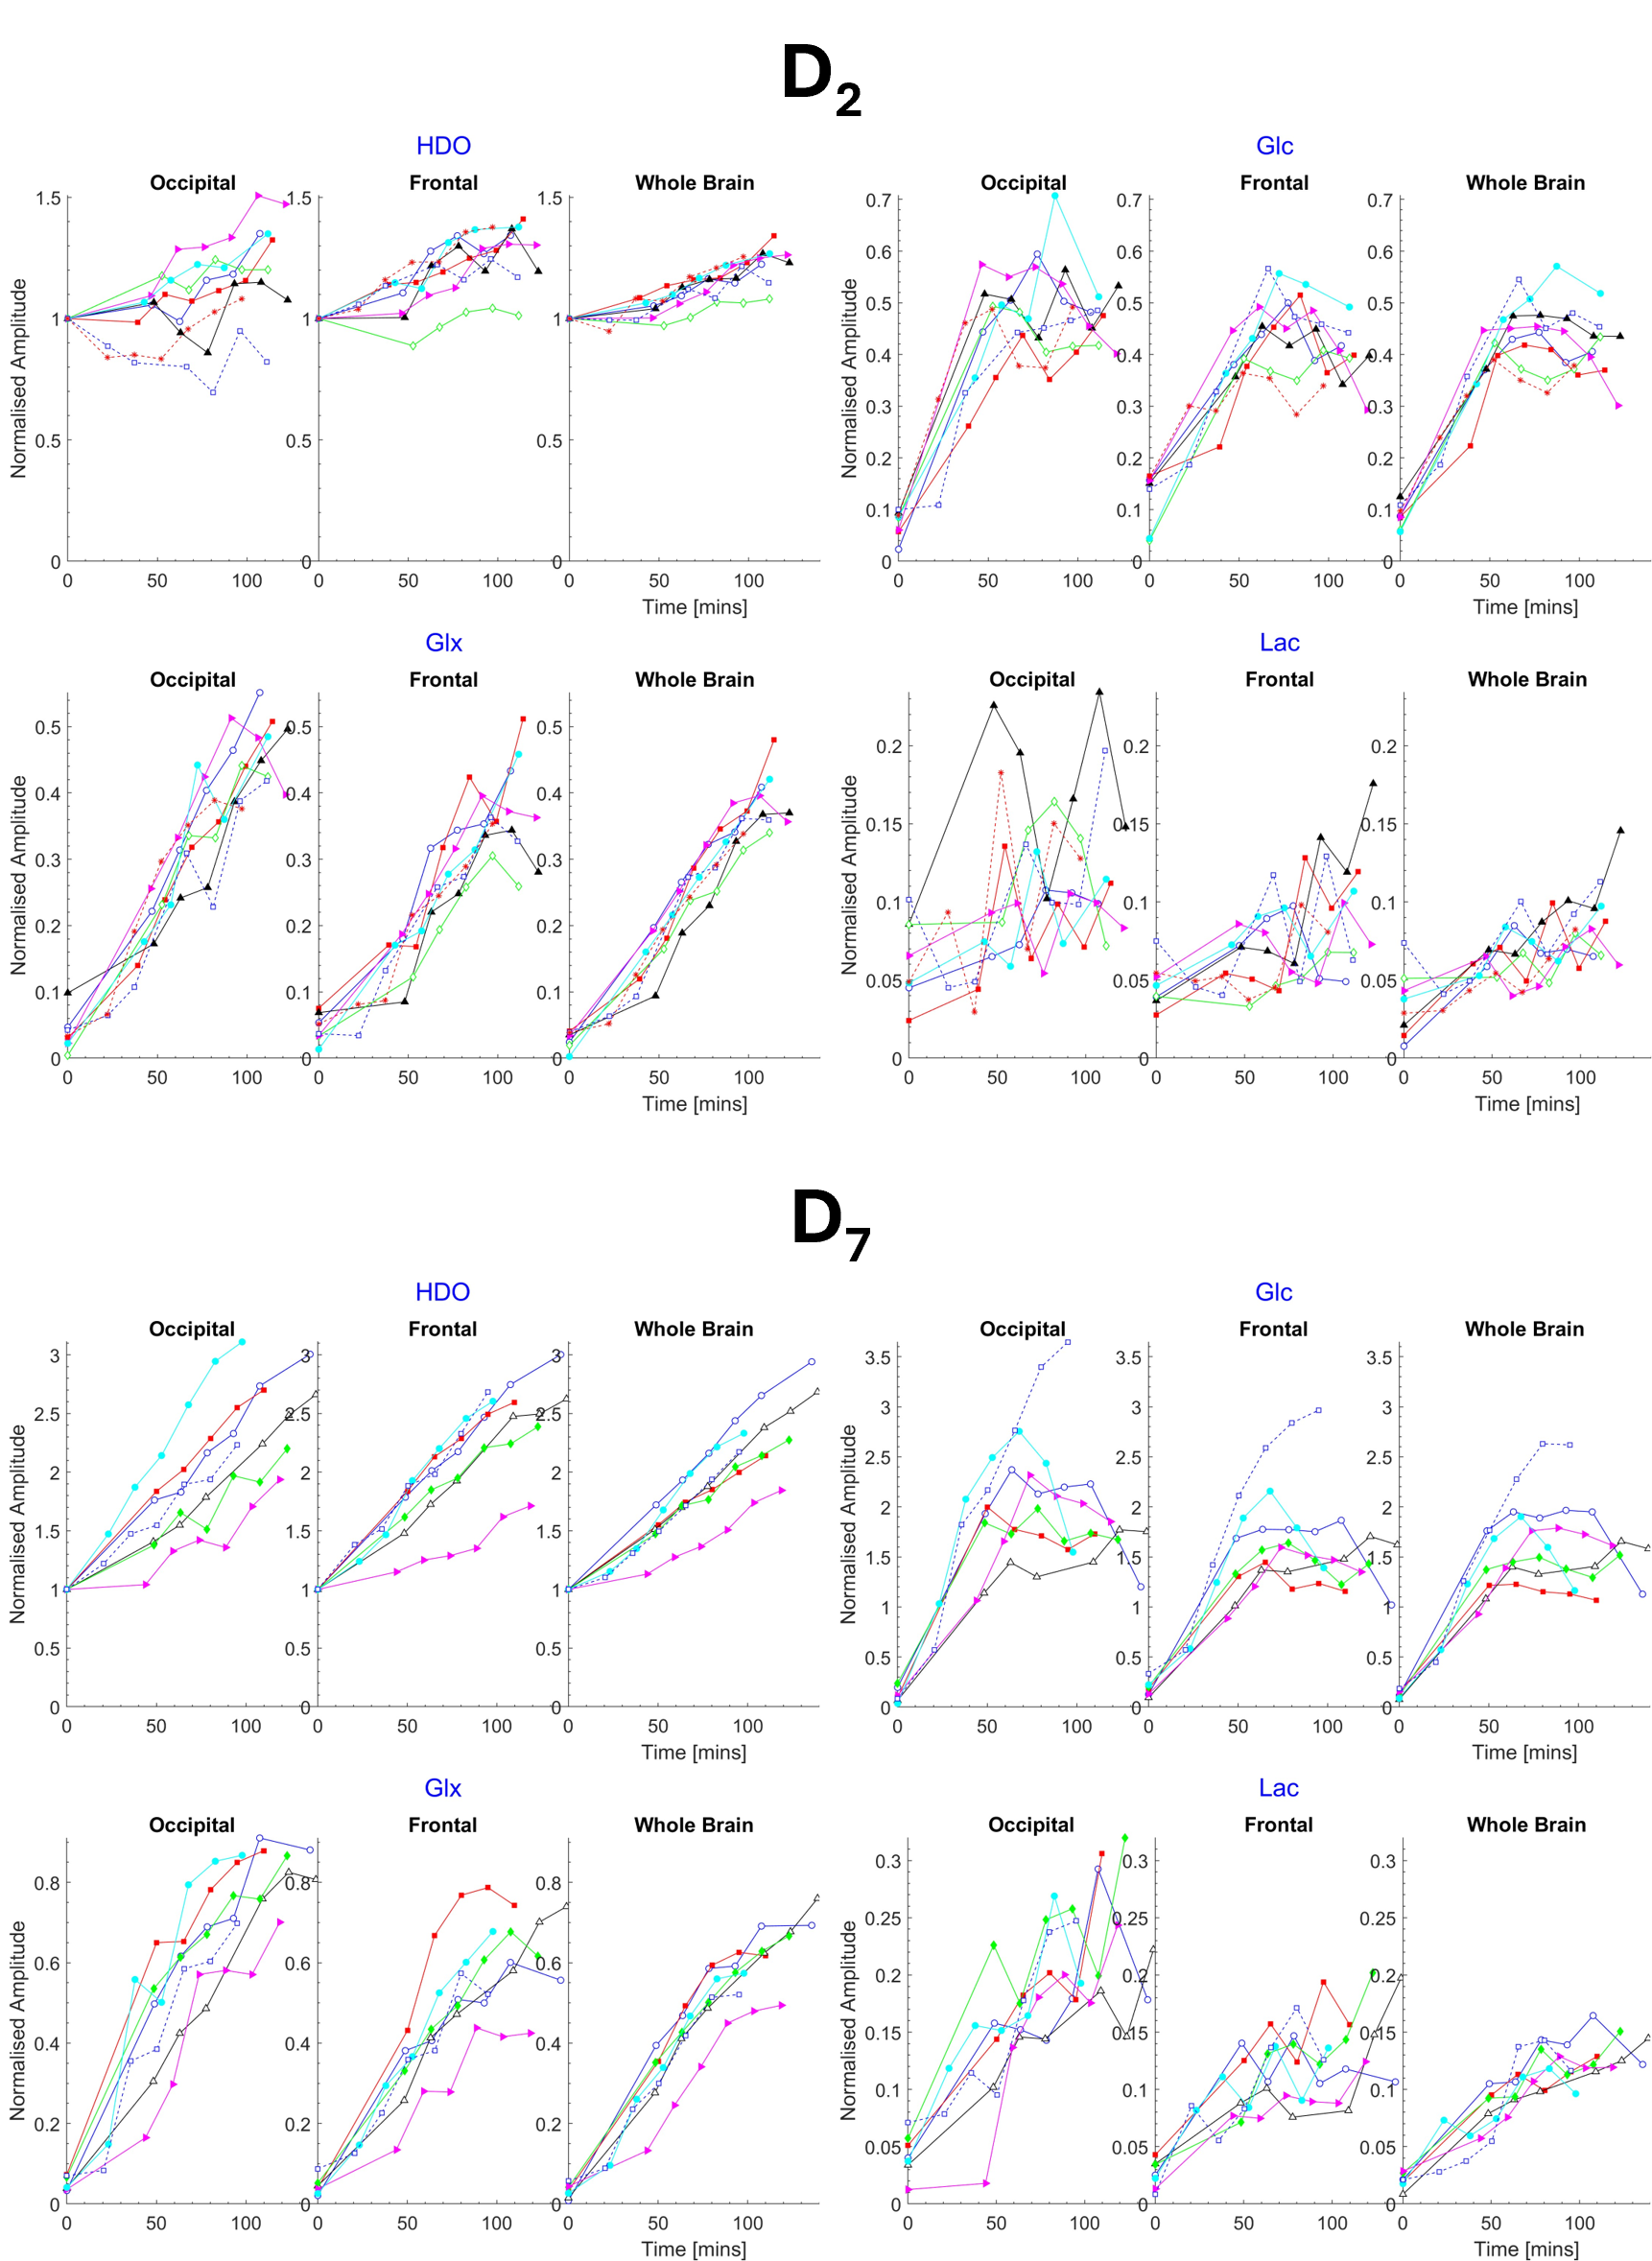
\includegraphics[width = 1\textwidth]{Figures/Glucose/Ind_Amp.png}
    \caption{\textit{Normalised metabolite signal amplitude time-courses for each participant for D$_2$-glucose (top) and D$_7$-glucose (bottom) for each \ac{ROI}: the occipital lobe, frontal lobe, and the whole brain.}}
    \label{fig:Glu:Ind_Amp}
\end{figure}

Figure \ref{fig:Glu:Avg_Amp} shows participant-averaged metabolite time-courses (non-averaged data are shown in Fig. \ref{fig:Glu:Ind_Amp}). These plots were generated by calculating the running average of the time-ordered data from all participants in the D$_2$ or D$_7$-glucose cohorts, with a window size equal to the number of participants in that cohort. This is shown in Fig. \ref{fig:Glu:Avg_Amp} with the errorbars being equal to the moving standard  amplitudes, here the metabolite signals are normalised to the \ac{HDO} signal at \ac{NA} obtained before ingestion of glucose, for each participant. The maximum in the averaged glucose signal is clearly visible and occurs between 50 and 100 minutes after glucose ingestion. In these plots, it is clear that all metabolite amplitudes from D$_7$-glucose ingestion are larger than those from D$_2$-glucose. 

\begin{figure}
    \centering
    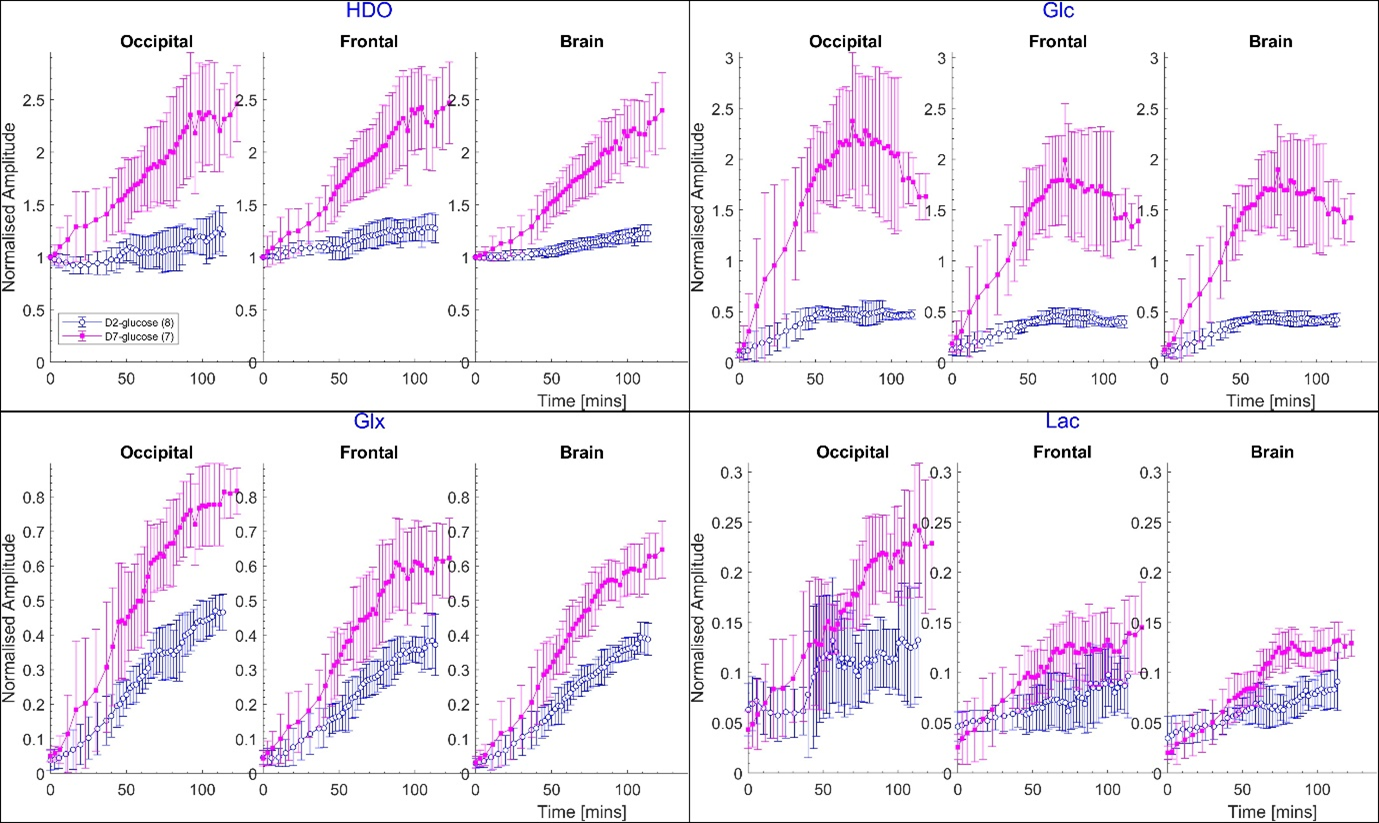
\includegraphics[width = 1\textwidth]{Figures/Glucose/Avg_Amp.png}
    \caption{\textit{Average time-courses of normalised metabolite signals for the occipital lobe, frontal lobe, and the whole brain from participants who ingested D$_2$-glucose (blue) and D$_7$-glucose (pink). A moving average which over the nearest points in time equal to the number of participants, with error bars representing the moving standard deviation.}}
    \label{fig:Glu:Avg_Amp}
\end{figure}

The same data, converted to concentrations are shown in Fig. \ref{eqn:Glu:Conc}. These concentrations have been corrected for label-loss, so that the values estimate the concentrations of deuterated molecules that would be observed if no label-loss occurred. As expected, the averaged concentrations of \ac{HDO}, Glx, and lactate are clearly different between the D$_2$ and D$_7$-glucose cohorts, with the glucose concentrations appearing similar. 

\begin{figure}
    \centering
    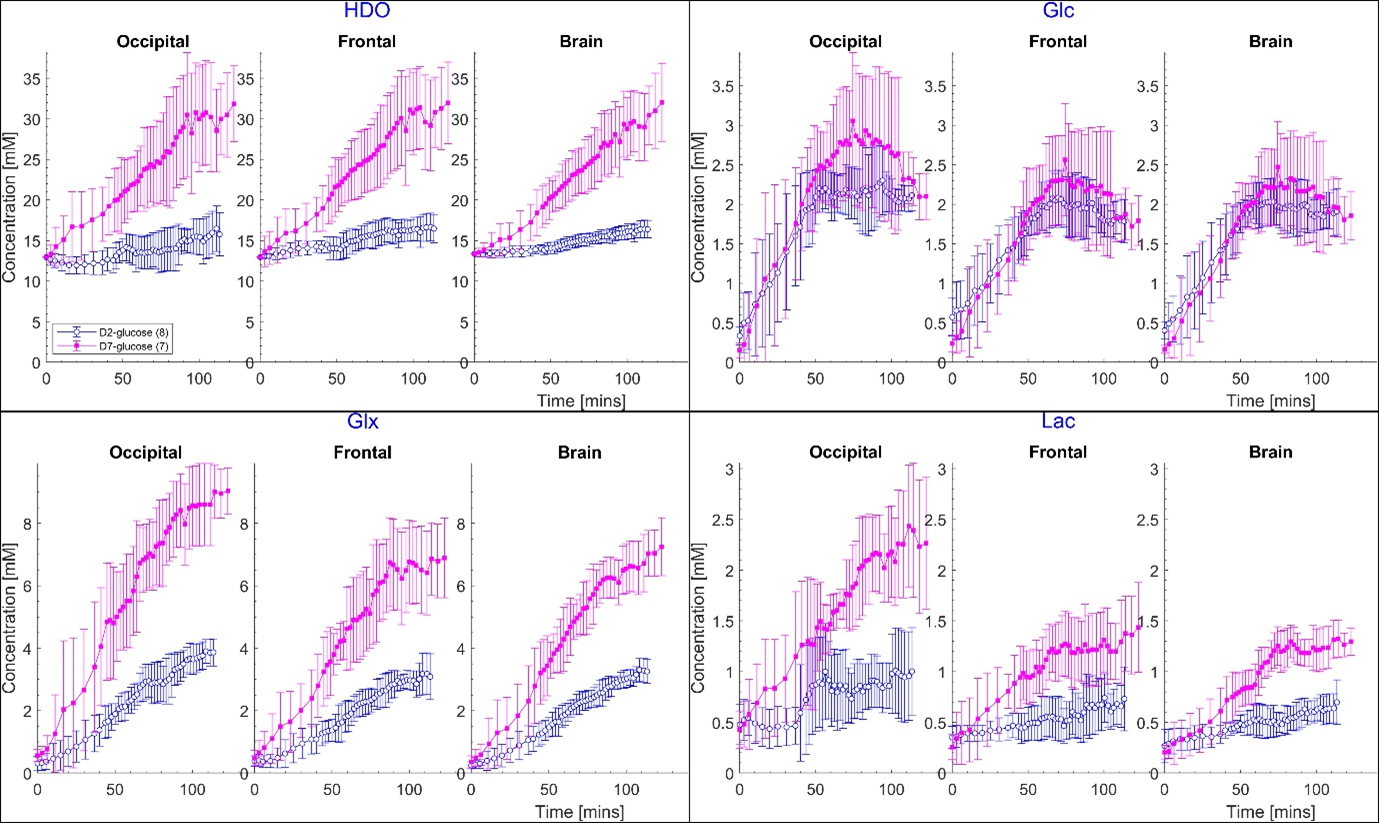
\includegraphics[width = 1\textwidth]{Figures/Glucose/Avg_Conc.png}
    \caption{\textit{Average time-courses of metabolite concentrations from the occipital lobe, frontal lobe, and the whole brain from participants who ingested D$_2$-glucose (blue) and D$_7$-glucose (pink). A moving average which over the nearest points in time equal to the number of participants, with error bars representing the moving standard deviation.}}
    \label{fig:Glu:Avg_Conc}
\end{figure}

To provide a clearer depiction of the relative metabolite signal amplitudes arising from D$_2$ and D$_7$-glucose ingestion, Fig. \ref{fig:Glu:D7_D2} shows plots of the ratios of metabolites from the two glucose isotopologues: Amplitude(D$_7$) / Amplitude(D$_2$). To calculate the ratio between the averaged D$_2$- and D$_7$-glucose signals, the data needs to cover the same points in time. Therefore, the D$_2$-glucose data is interpolated to the same time series data as the D$_7$-glucose data. The error bars are derived from the error bars (standard deviations) of the numerator and denominator by the standard method of combining independent errors of a quotient. 

\begin{figure}
    \centering
    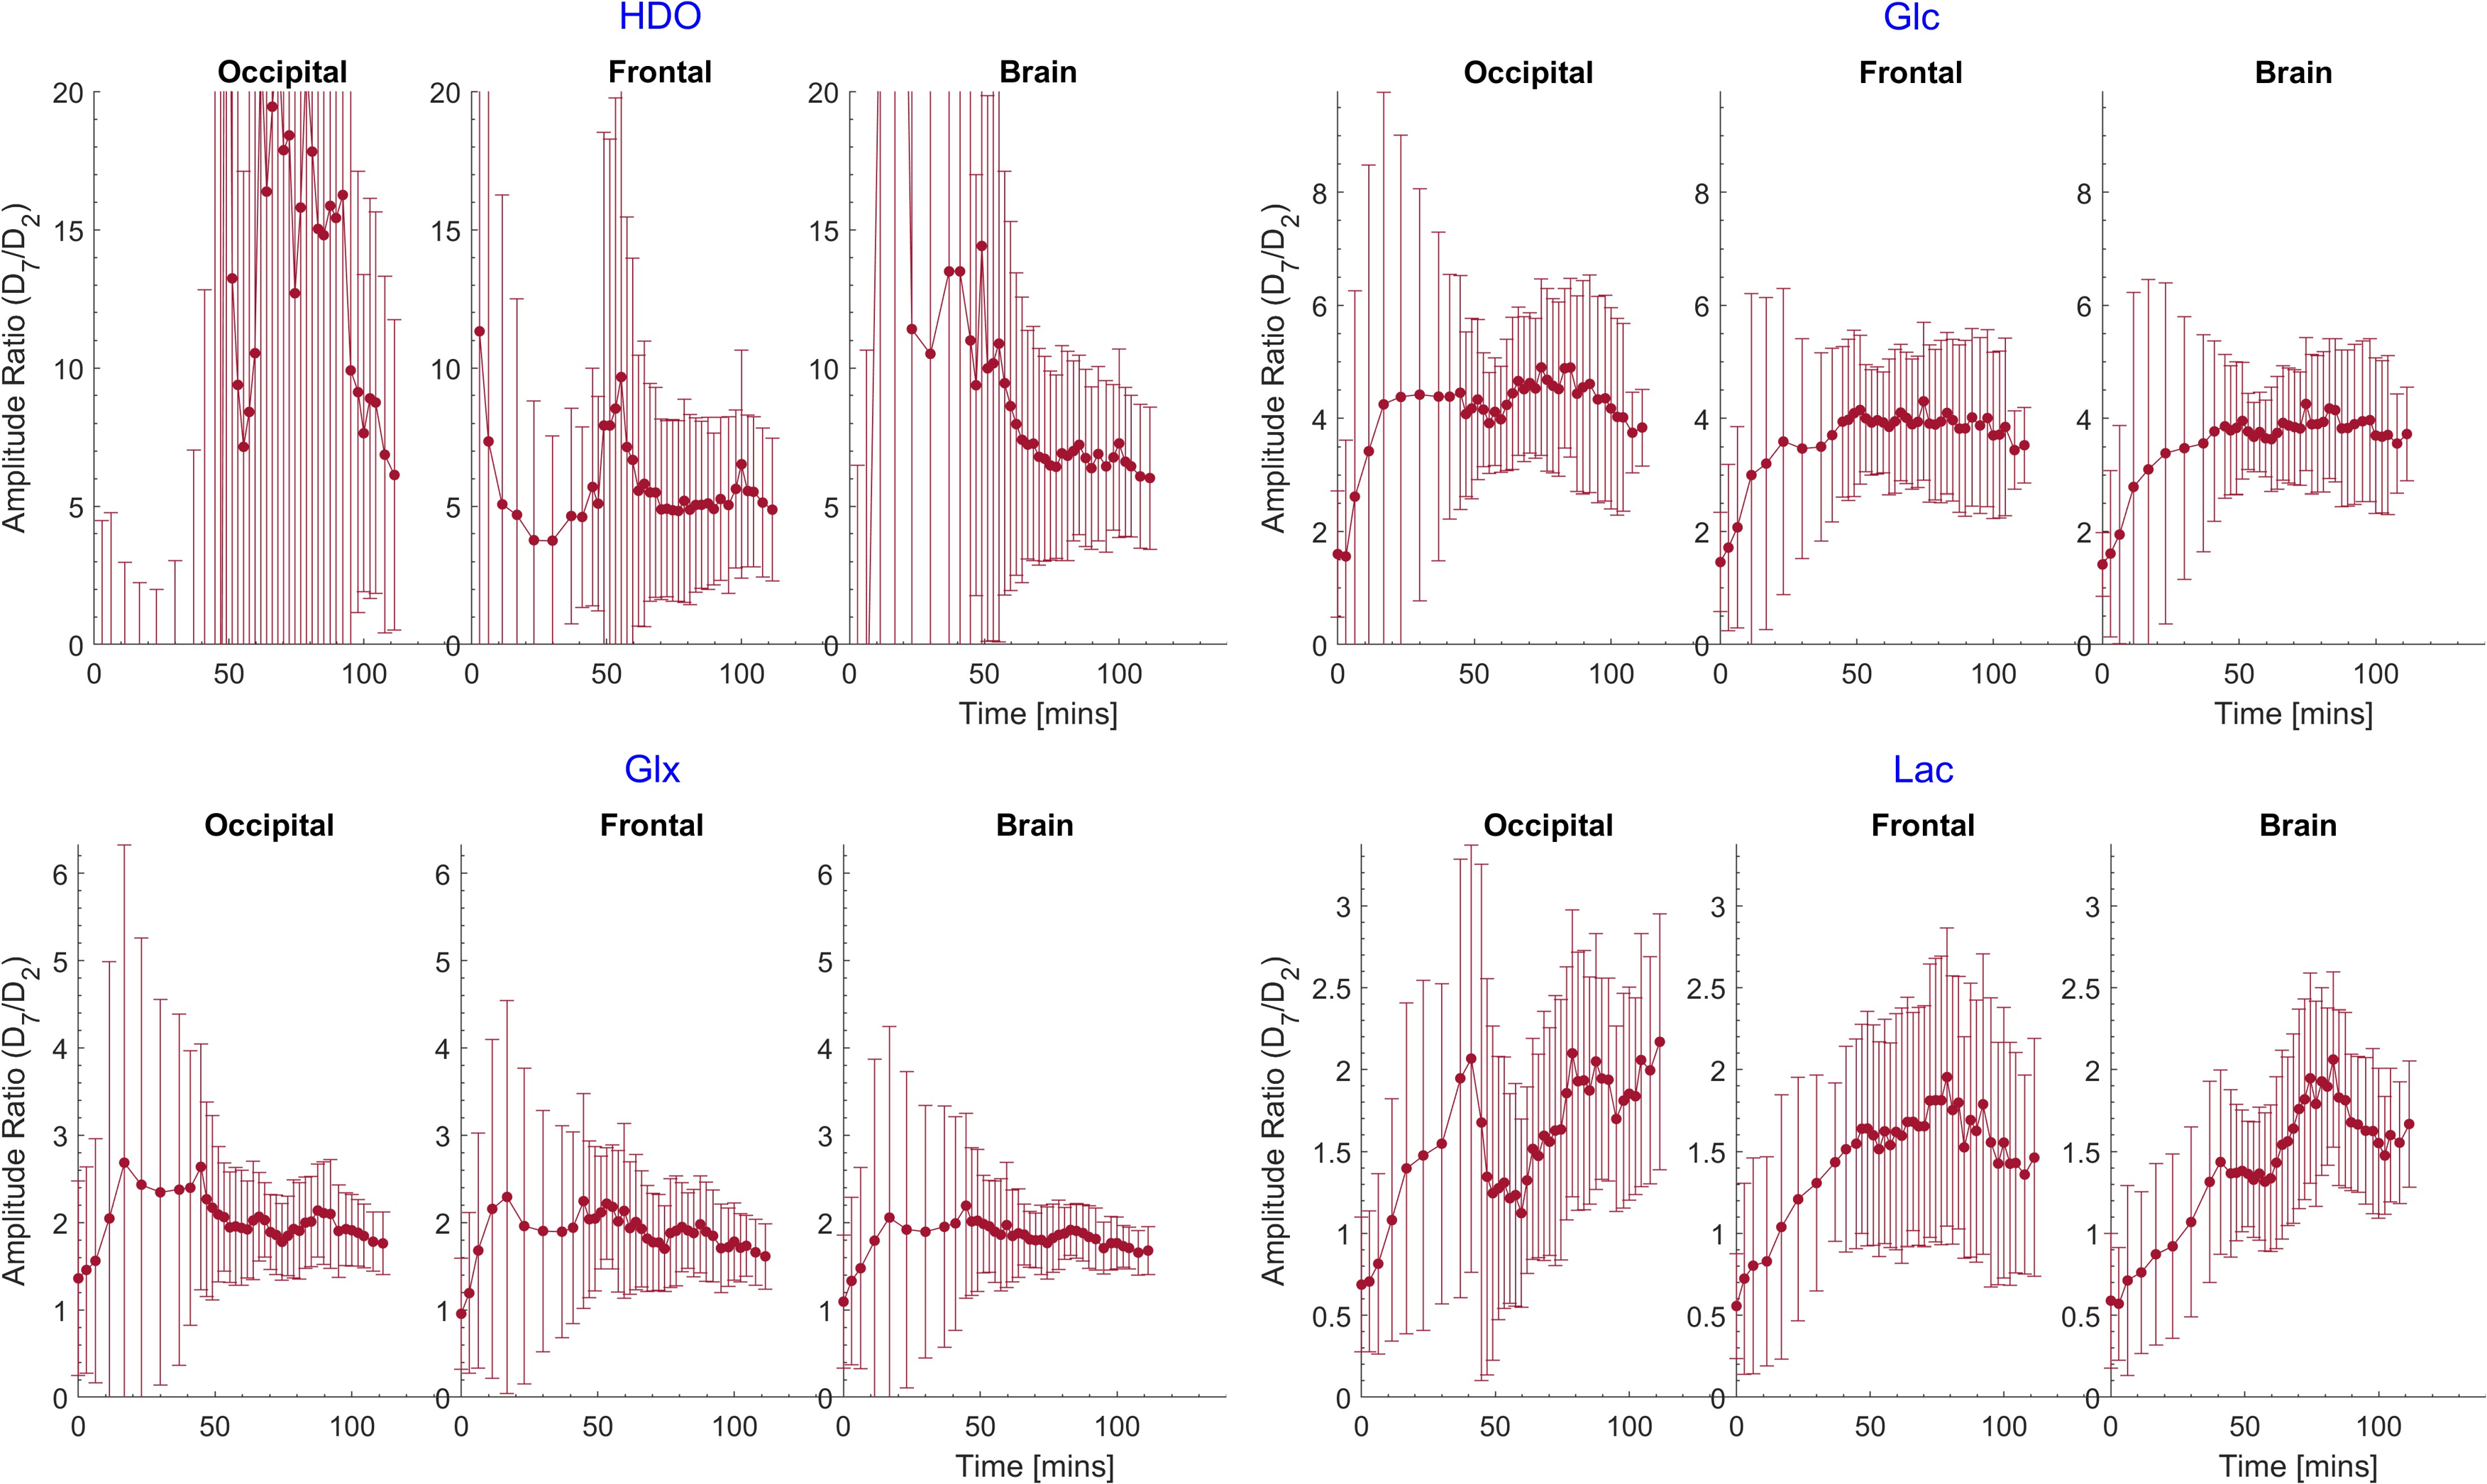
\includegraphics[width = 1\textwidth]{Figures/Glucose/D7_D2.png}
    \caption{\textit{Normalised signal intensity ratios for each metabolite of D$_7$- to D$_2$-glucose for the same regions in Fig. \ref{fig:Glu:Avg_Conc}. The D$_7$-glucose data is interpolated (after the moving average in Fig. \ref{fig:Glu:Avg_Conc}. is applied) to the same time-course as the D$_2$-glucose data before the ratio calculation. The amplitude of the errorbars are now the previous standard deviations of the numerator and denominator combined by using the standard method of combining independent errors of a quotient.}}
    \label{fig:Glu:D7_D2}
\end{figure}

In the plots for \ac{HDO}, the \ac{NA} values have been subtracted to produce a ratio of the \ac{HDO} increases above \ac{NA}. Although there is considerable variability, focussing on the whole-brain \ac{ROI} (which should possess the best \ac{SNR}), it appears that the ratios are converging to approximately constant values, such that for \ac{HDO}, glucose, Glx, and lactate, the ratios are 5.5 $\pm$ 2.5, 3.5 $\pm$ 1.0, 1.6 $\pm$ 0.4, and 1.5 $\pm$ 0.4, respectively. It has been previously suggested that \ac{HDO} production from the metabolism of D$_7$-glucose can be used as a biomarker \cite{Mahar2021DeuteratedGlucose}, that the ratio $\Delta$HDO/(Glx+Lac) of T$_1$-corrected signal amplitudes (where $\Delta$HDO is the increase in labelled water above \ac{NA}) has a quasi-stable value of 2.5, calculated by taking account of label-loss from Glx and lactate, and label-gain to \ac{HDO}. This ratio is shown in Fig. \ref{fig:Glu:HDO_Rat} as well as similar plots for glucose, Glx, and lactate, for both D$_2$ and D$_7$-glucose. The plots of $\Delta$HDO/(Glx+Lac) for D$_7$-glucose appear to also show a quasi-stable region, although at values $<$2.5. Plots for Glx/(Glx+Lac) appear to show long-time convergence to approximately 0.8 which is similar to what has been shown previuosly \cite{Kaggie2022DeuteriumMetabolism}, for both D$_2$ and D$_7$-glucose. However, Glc/(Glx+Lac) plots show global maxima at approximately 30 – 70 minutes, and appear to occur earlier than the maxima of glucose in the plots of Figs. \ref{fig:Glu:Avg_Amp} and \ref{fig:Glu:Avg_Conc}.  

\begin{figure}
    \centering
    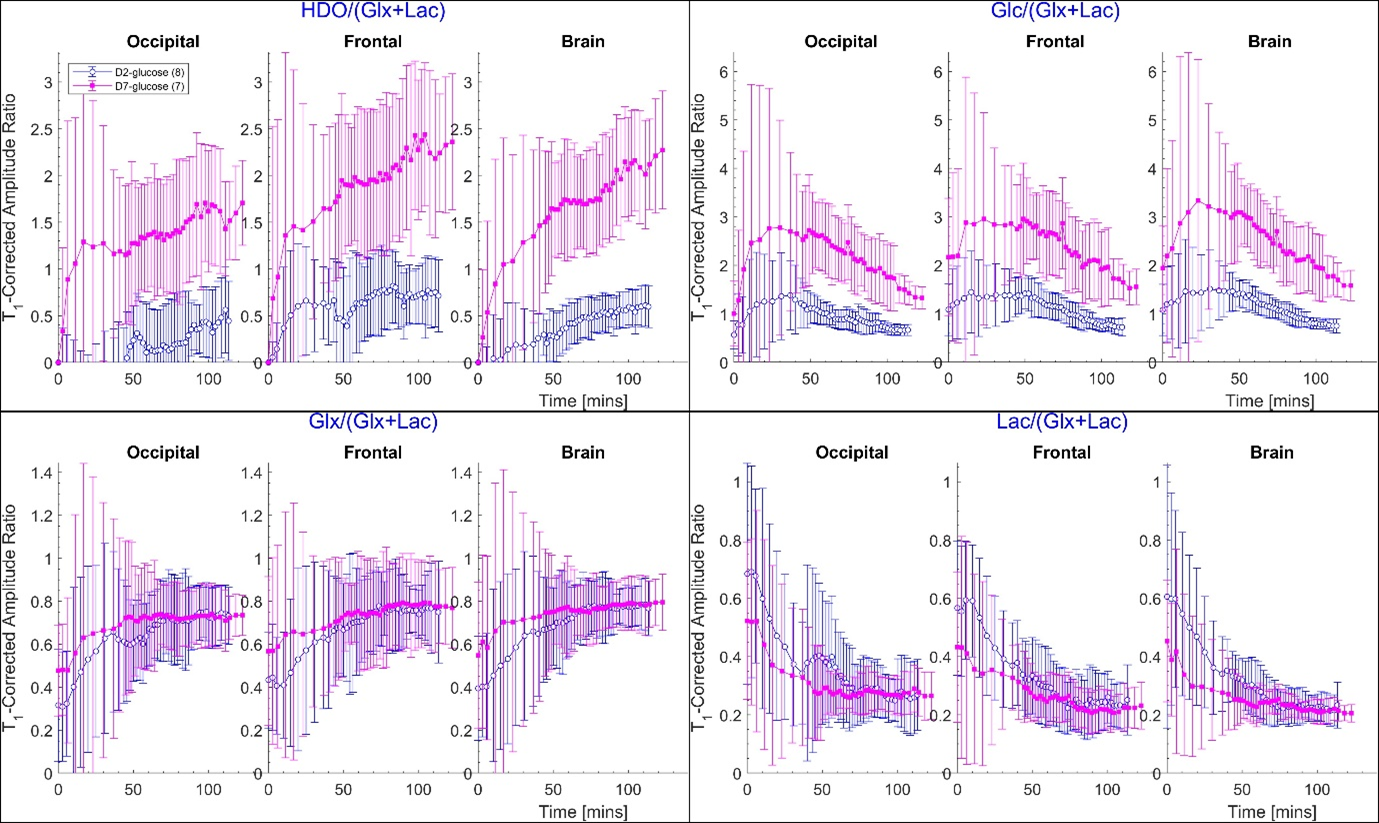
\includegraphics[width = 1\textwidth]{Figures/Glucose/HDO_Ratio.png}
    \caption{\textit{Ratio of each metabolite signal to the sum of downstream metabolites (Glx and lactate) for the same regions in Fig. \ref{fig:Glu:Avg_Conc}. The D$_7$-glucose data is interpolated (after the moving average in Fig. \ref{fig:Glu:Avg_Conc}. is applied) to the same time-course as the D$_2$-glucose data before the ratio calculation. The amplitude of the errorbars are now the previous standard deviations of the \ac{HDO} amplitude and the denominator combined by the standard method of combining independent errors of a quotient.}}
    \label{fig:Glu:HDO_Rat}
\end{figure}

\section{Discussion}

$^2$H spectra and \ac{CSI} data were acquired from fifteen participants, who had ingested either D$_2$- or D$_7$-glucose, before and then at 5 or 6 time points after consumption spanning around 90 minutes, with nine of these participants experiencing visual stimulation during the \ac{CSI} scans. In all spectra, after glucose ingestion, deuterated water (\ac{HDO}), non-metabolised glucose, and Glx were detected for both glucose isotopologues. Lactate was also detected in most spectra but was present in lower concentrations, particularly for D$_2$-glucose, and was generally more challenging to detect, although average time-courses from all participants revealed an unambiguous accumulation of a deuterated substance at the lactate resonance (see Figs. \ref{fig:Glu:Avg_Amp} and \ref{fig:Glu:Avg_Conc}). However, no effect of visual stimulation could be discerned, either in comparison to participants who did not undergo visual stimulation as can be seen in Fig. \ref{fig:Glu:Vis_Stim} or in comparing metabolite accumulations between frontal and occipital lobes as can be seen in Fig. \ref{fig:Glu:Avg_Conc}.

\begin{figure}
    \centering
    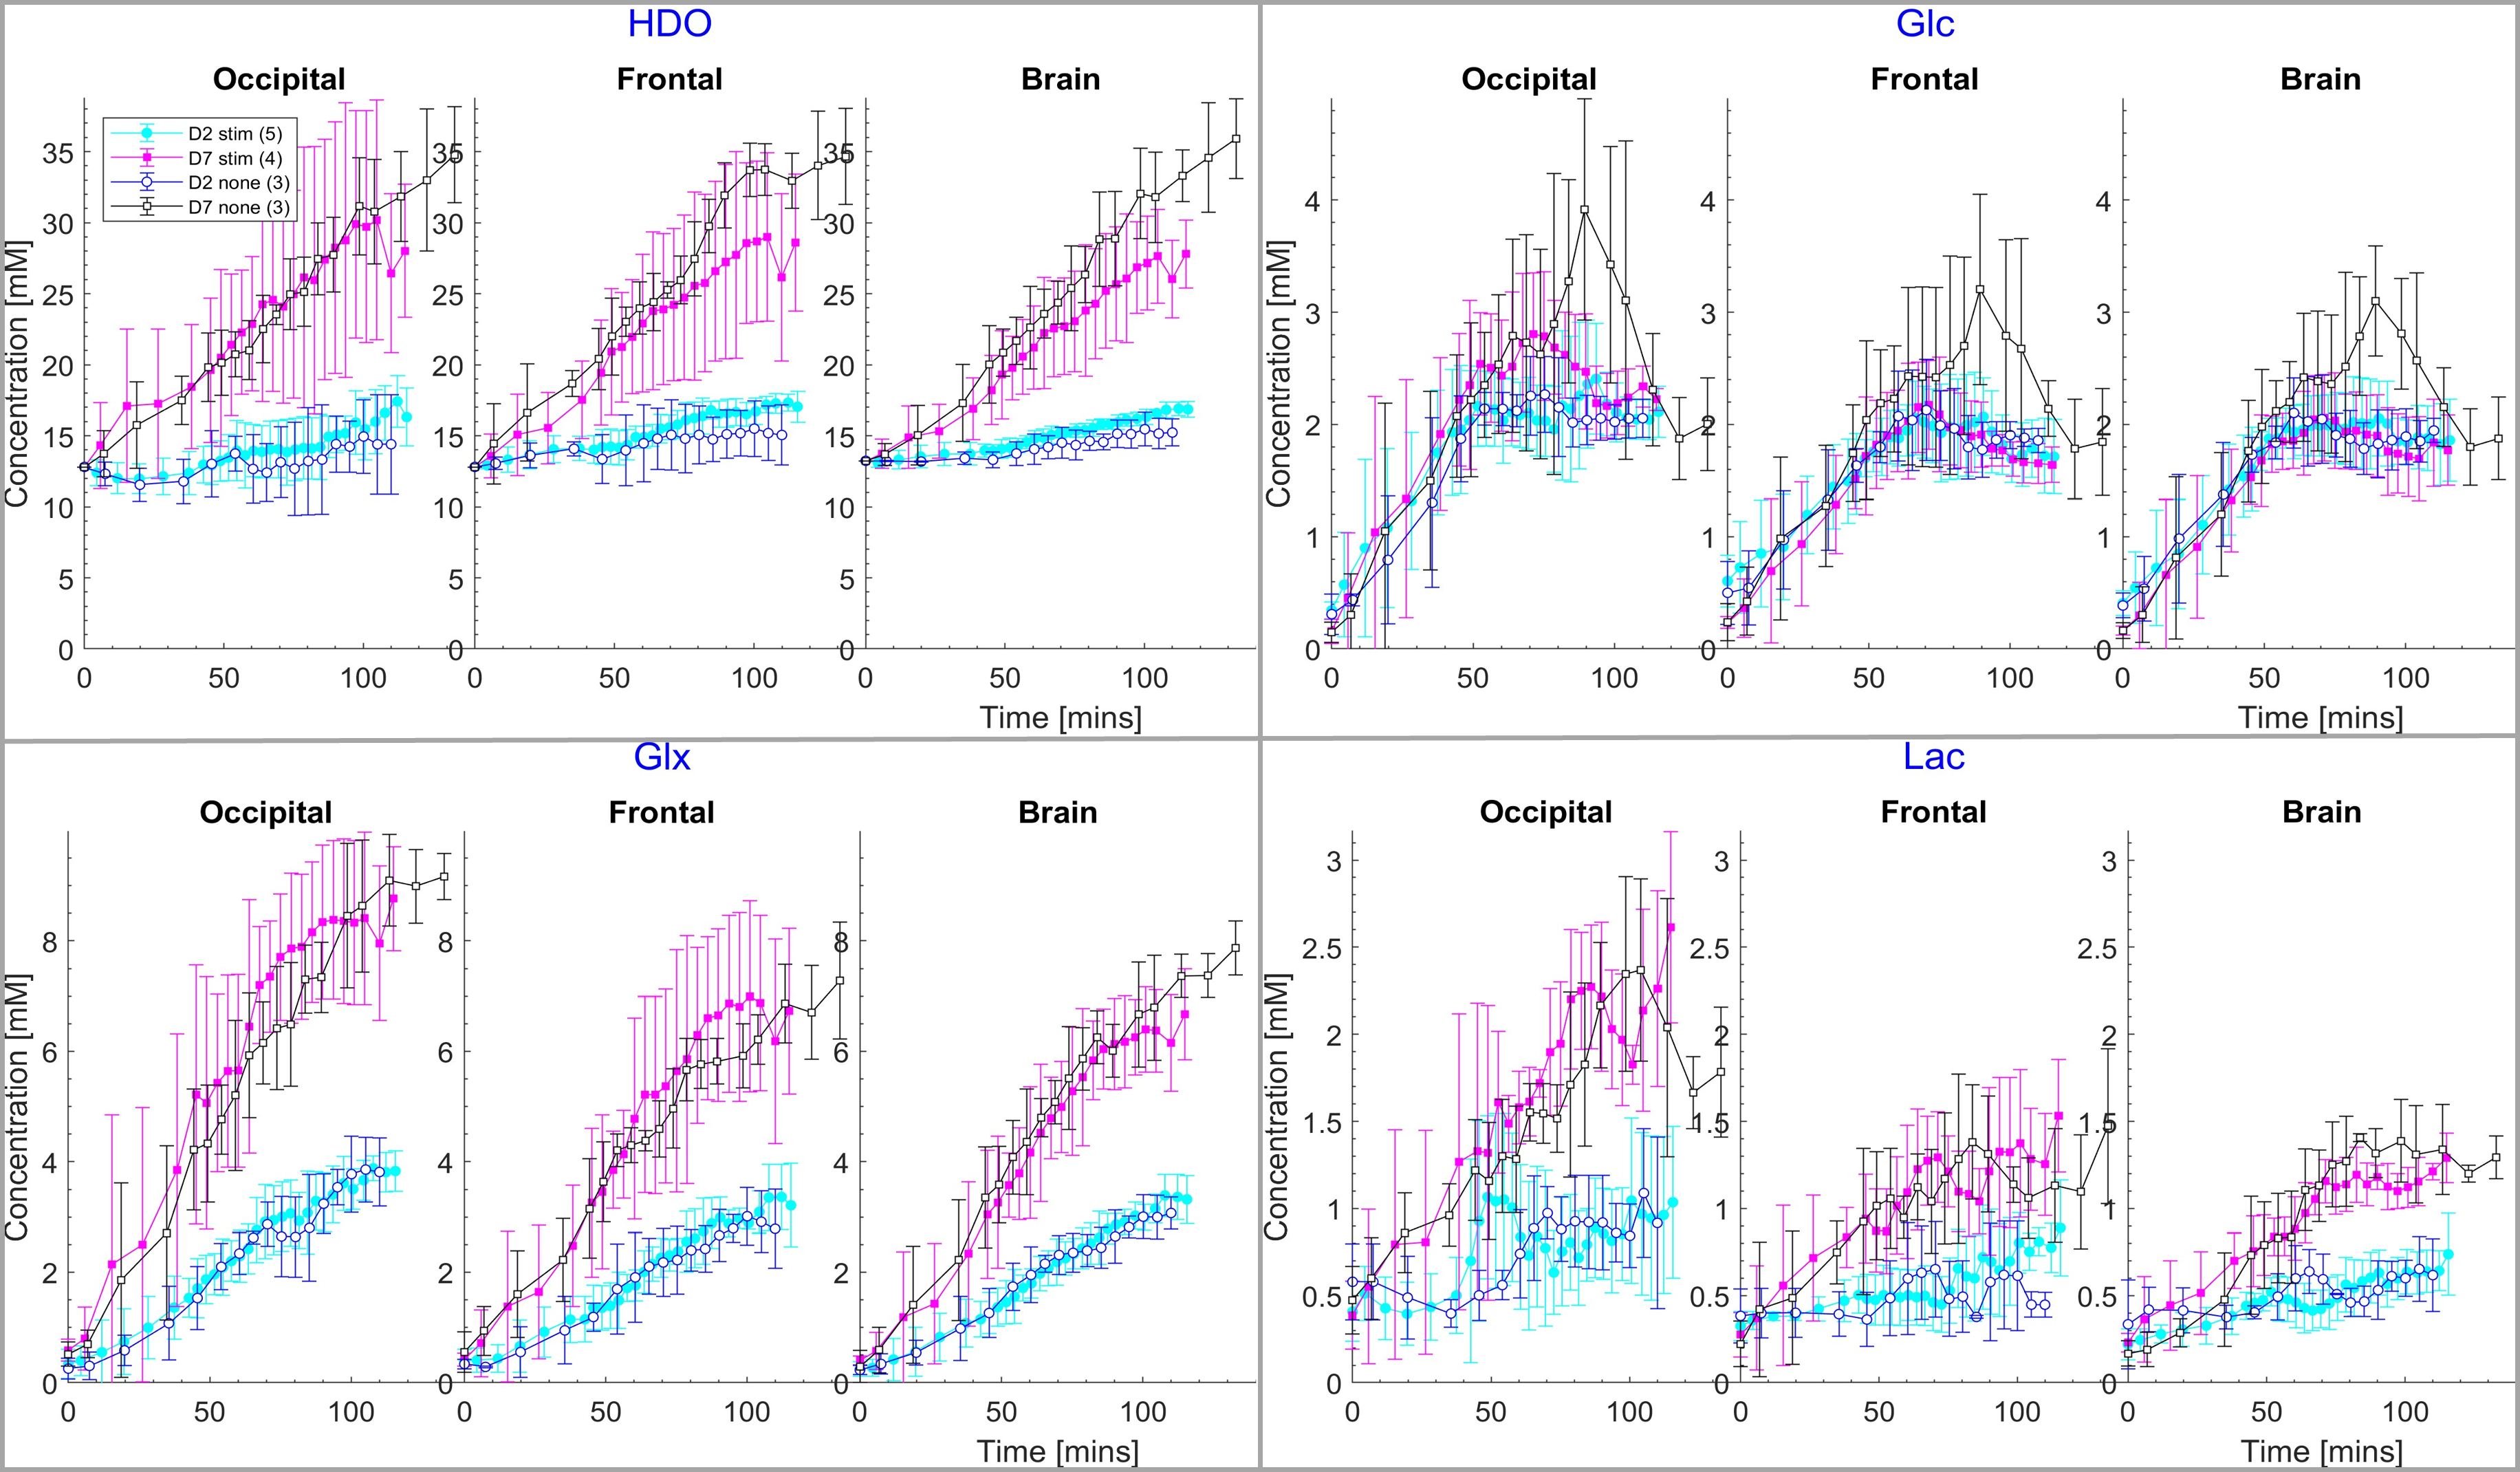
\includegraphics[width = 1\textwidth]{Figures/Glucose/Vis_Stim.png}
    \caption{\textit{Average time-courses of metabolite concentrations from the occipital lobe, frontal lobe, and the whole brain from participants who ingested D$_2$-glucose and had no visual stimulus (blue) and those who were visually stimulated (light-blue) along with those who ingested D$_7$-glucose and had no visual stimulus (black) and those were visually stimulated (pink). A moving average which over the nearest points in time equal to the number of participants, with error bars representing the moving standard deviation.}}
    \label{fig:Glu:Vis_Stim}
\end{figure}

 Compared to the \ac{CSI} data, slice-selective deuterium spectra can be acquired in a much shorter time and the higher \ac{SNR} can provide a more reliable analysis if the magnetic field homogeneity is adequate to provide a reasonable linewidth. Such spectra are displayed in Fig. \ref{fig:Glu:Select}, showing their time evolution from \ac{NA} to over 100 minutes after glucose ingestion. HDO (4.8 ppm), glucose (approximately 3.8 ppm), and Glx (2.4 ppm) are clearly visible in these spectra, with amplitudes being generally larger for the spectra of the participant who ingested D$_7$-glucose, especially for the \ac{HDO} peak. Although possessing a very low \ac{SNR}, a peak at 1.3 ppm is just visible in some of these spectra and, again, generally appears to be larger in the D$_7$-glucose spectra. The fact that it is larger in the D$_7$-glucose spectra suggests that it is a result of lactate accumulation but could also contain a \ac{NA} lipid component arising from the skull. Examples of spectral fits are shown in Fig. \ref{fig:Glu:Select} for the last time-point spectra in the two displayed data sets. Here it can be seen that spectral components, including the anomeric decomposition of the two glucose isotopologues, fit well with small residuals.

\ac{CSI} \ac{SNR} can be improved by increasing the number of averages as opposed to acquiring multiple \ac{CSI} data sets at different time points. However, by acquiring metabolite time-courses the time point at which the signal from glucose (and other metabolites) is largest signal maximises can be found. Time-course data can also be used to model the data. Metabolic modelling has previously been attempted with pre-clinical data \cite{Lu2017QuantitativeSpectroscopy, Rich20201HVivo, Kreis2020MeasuringMRI, Simoes2022GlucoseGlioblastoma}. Only recently modelling been used with human data where D$_2$-glucose was ingested orally \cite{Ruhm2022Dynamic9.4T} as opposed to intravenous infusion which is used in animal models. An estimate of the data quality that would have been obtained if only a single \ac{CSI} was acquired with a higher number of averages can be obtained by combining several of the \ac{CSI} acquisitions into single data-sets. Figs. \ref{fig:Glu:D2_CSI} and \ref{fig:Glu:D7_CSI} demonstrate the result of doing this for D$_2$ and D$_7$-glucose data where six consecutive post-glucose-ingestion \ac{CSI} acquisitions are combined. This would approximately correspond to a single acquisition with 36 averages for a total scan duration of 57 minutes, although this duration is due to the full use of acquisition-weighted averaging \cite{Pohmann2001AccurateCSI}, usually this would take 125 minutes. The spectra shown, from a single voxel in the averaged \ac{CSI}, has the same essential features as the slice-selective spectra in Fig. \ref{fig:Glu:Select}; clear \ac{HDO}, glucose, and Glx peaks, with small low-\ac{SNR} peaks where lactate is expected. In this case, it is less likely that these peaks contain a large lipid contribution, which suggests they arise from lactate. 

% From \ref{fig:Glu:CSI} it is evident that the metabolite signals are hyperintense in the cortex of the brain with the lateral ventricles appearing hypointense. This is consistent with previous work at ultra-high field12,13 this has been difficult to show as more advanced multi-channel coils tend to be more sensitive to the peripheral regions of the brain anyway, however we are using a single-channel birdcage coil which is more sensitive in the centre of the brain. To overcome this issue previous work has shown metabolic maps divided by the HDO signal as it was said to be a good estimate of B1 homogeneity, however, it is shown here that this is not the case here as both types of glucose have distinct metabolic fluxes in HDO signal (D$_7$-glucose being much more metabolically active). 

The resolution of the \ac{CSI} data acquired here is too low to be able to differentiate \ac{GM} and \ac{WM} in the cortex after interpolation. \ac{ROI}-averaged metabolite amplitudes from individual participant data sets were often noisy and their underlying time-dependence could be obscured see Fig. \ref{fig:Glu:Ind_Amp}. This was more often the case for participants who ingested D$_2$-glucose, whose metabolite amplitudes tended to be lower, but was also an issue for the lactate signal for both glucose isotopologues. Averaging the data over all participants, however, as is presented in Fig. \ref{fig:Glu:Avg_Amp}, delivered a clearer picture of the temporal accumulation of the deuterated metabolites. The curves for glucose clearly reach a global maximum within the timeframe of the experiments, and \ac{HDO}, Glx, and lactate, all unambiguously show increasing amplitudes over time. The increases in \ac{HDO} and Glx are as expected from many previous studies, but the observation of an increase in lactate is less common, although it has also been previously measured  \cite{Ruhm2021DeuteriumResolution, Kaggie2022DeuteriumMetabolism}. 

% It has been shown that the apparent lactate curve probably consists of a non-zero lipid component that possibly has a small time-dependence, plus a small lactate component with a larger time-dependence \cite{Ruhm2021DeuteriumResolution}.     

No significant difference for any metabolite (\ac{HDO}, Glc, Glx, and Lac) was seen between participants that had a visual stimulus applied and those that did not. One could compare the metabolism in the frontal lobe and the occipital lobe, however there was also a notable difference between the regions in participants who did not have visual stimulus applied. Because of the time-course that goes from no detectable signal in glucose, Glx and lactate to a detectable signal it is difficult to compare any other changes above the inter-participant variability which can be larger than 10\%. However, it is easier to see metabolite changes in response to visual stimulus using other nuclei such as $^{13}$C, $^{31}$P and $^1$H as there is already baseline measurements so changes are easier to detect. Also, even after a long period the lactate signal is still difficult to detect and fit, so any additional changes are difficult to detect.  

One of the reasons for the large inter-participant variability across all subjects is the evident ‘decrease’ between \ac{NA} and the first two time points in all metabolite concentrations, most evidently in HDO. This is because at early time points the metabolism has not had long enough accumulate increased concentrations that would dominate the variability arising from small differences in head position after repositioning in the scanner. The low \ac{SNR} of the anatomical $^1$H \ac{MPRAGE} scan that was acquired could also mean that the \ac{ROI}s could be better defined and represent the regions more accurately. This is backed up by the largest ROI of the whole brain suffering from this effect the least. Availability of more sophisticated multi-channel RF coil would help mitigate this problem and lead to better \ac{ROI}s.

The differences in the steady-state signal between the D$_2$- and D$_7$-glucose datasets are similar to what has been theorised from animal models \cite{Mahar2021DeuteratedGlucose}. These values can slightly alter due to hydrogen-deuterium exchange but ultimately remain stable. They can also change due to label loss, which has been measured in rat models and shown to be stable which means it can be accounted for \cite{DeGraaf2021CharacterizationStudies}. The increase in \ac{HDO} signal that is generated from the label loss has been quantified in D$_7$-glucose approximately six times when compared to D$_2$-glucose. It has already been shown that the increase in \ac{HDO} for D$_7$-glucose is an appropriate measure for Warburg metabolism, as the glucose consumption is directly correlated HDO production30. However, the ratio between \ac{HDO} and Glx +lactate is much higher in literature ($\approx$2.5) than compared to this study ($\approx$1.5), however it is still evident as shown in Fig. \ref{fig:Glu:HDO_Rat}. The difference in ratio could come from the difference in infusion techniques, or it could result from differing amount of label loss.

\section{Conclusion}

This study has shown the first in vivo studies in human participants using D$_7$-glucose to track metabolism in the brain. Multiple $^2$H \ac{CSI} data was obtained over different time points was obtained and changes in metabolite (\ac{HDO}, Glu, Glc and Lac) are tracked over time. Postprocessing de-noising is used to increase \ac{SNR} for each dataset, acquisition based averaging is also used and could be extended to increase \ac{SNR} further at the expense of number of time points. D$_7$-glucose has been shown to offer an opportunity to improve the visualisation of Warburg metabolism \textit{in vivo} for patients, by increasing the signal of all available metabolites compared to D$_2$-glucose. 